\documentclass[11pt,letterpaper]{article}

\usepackage[utf8]{inputenc}
\usepackage[T1]{fontenc}
\usepackage{lmodern}
\usepackage[margin=1in]{geometry}
\usepackage{amsmath,amssymb,amsfonts}
\usepackage{graphicx}
\usepackage{booktabs}
\usepackage{longtable}
\usepackage{array}
\usepackage{multirow}
\usepackage{xcolor}
\usepackage{hyperref}
\usepackage{cleveref}
\usepackage{caption}
\usepackage{subcaption}
\usepackage{float}
\usepackage{setspace}
\usepackage{fancyhdr}
\usepackage{tikz}
\usetikzlibrary{arrows.meta,positioning,shapes.geometric,fit,backgrounds}

\definecolor{OkabeBlue}{HTML}{0072B2}
\definecolor{OkabeOrange}{HTML}{D55E00}
\definecolor{OkabeGreen}{HTML}{009E73}
\definecolor{OkabePurple}{HTML}{CC79A7}
\definecolor{OkabeGray}{HTML}{555555}
\definecolor{BoxBg}{HTML}{F7F9FB}

\hypersetup{
  colorlinks=true,
  linkcolor=OkabeBlue,
  citecolor=OkabeBlue,
  urlcolor=OkabeBlue,
  pdftitle={Medical Domain Adaptation and Clinical Integration: Transferring Sequence Modeling Techniques to Dermatoscopic Skin Lesion Diagnosis},
  pdfauthor={Group 8 -- Machine Learning 2026-III, Universidad Distrital Francisco Jose de Caldas}
}

\pagestyle{fancy}
\fancyhf{}
\lhead{\small\textsc{Machine Learning 2026-III -- Workshop No. 6 (Group 8)}}
\rhead{\small\textsc{Medical Domain Adaptation \& Clinical Integration}}
\cfoot{\thepage}
\setlength{\headheight}{14pt}
\onehalfspacing

% Safe figure inclusion: renders real 300-dpi figure when generated by run_all_rocm.sh
\newcommand{\safeincludegraphics}[3][0.95\textwidth]{%
  \IfFileExists{#2}{%
    \includegraphics[width=#1]{#2}%
  }{%
    \fcolorbox{OkabeGray}{BoxBg}{%
      \begin{minipage}[c][4.2cm][c]{0.88\textwidth}
        \centering
        \textbf{Pending Figure Artifact:} \texttt{\detokenize{#2}}\\[4pt]
        \small #3\\[4pt]
        \footnotesize Execute \texttt{bash Workshop\_6/scripts/run\_all\_rocm.sh} on AMD RX 9060 XT (ROCm) to generate and embed this figure automatically.
      \end{minipage}%
    }%
  }%
}

% Auto-generated by Workshop_6/src/build_report_assets.py — DO NOT EDIT BY HAND
\newcommand{\WFiveNoiseFOne}{0.3412}
\newcommand{\WFiveRealBPC}{1.8233}
\newcommand{\WFiveVanillaPPL}{83.42}
\newcommand{\WFiveWGANBPC}{1.8179}
\newcommand{\WFiveWGANPPL}{20259.0}
\newcommand{\WFourAEAcc}{81.1\%}
\newcommand{\WFourVAEAcc}{65.2\%}
\newcommand{\WFourVAEAnomFOne}{0.9995}
\newcommand{\WOneLogAcc}{30.2\%}
\newcommand{\WOneLogBPC}{3.620}
\newcommand{\WOneLogFOne}{0.1222}
\newcommand{\WOneNBAcc}{33.5\%}
\newcommand{\WOneNBFOne}{0.0711}
\newcommand{\WSixBestBalAcc}{0.765}
\newcommand{\WSixBestECE}{0.0257}
\newcommand{\WSixBestMalAUC}{0.925}
\newcommand{\WSixBestMalPRAUC}{0.758}
\newcommand{\WSixBestModel}{a1\_resnet18\_imagenet\_finetune}
\newcommand{\WSixBestSensScr}{96.0\%}
\newcommand{\WSixBestSensYouden}{92.0\%}
\newcommand{\WSixBestSpecScr}{67.0\%}
\newcommand{\WSixBestSpecYouden}{78.0\%}
\newcommand{\WSixTestImgs}{1,496}
\newcommand{\WSixTestLesions}{1,121}
\newcommand{\WSixTrainImgs}{7,000}
\newcommand{\WSixTrainLesions}{5,228}
\newcommand{\WSixValImgs}{1,519}
\newcommand{\WSixValLesions}{1,121}
\newcommand{\WSixXaiBorderEnergy}{8.4\%}
\newcommand{\WSixXaiIoU}{0.348}
\newcommand{\WSixXaiLesionEnergy}{49.3\%}
\newcommand{\WSixXaiPointingAcc}{73.3\%}
\newcommand{\WThreeDQNInvalid}{0.1\%}
\newcommand{\WThreeDQNNewWord}{92.8\%}
\newcommand{\WThreeDQNReturn}{+1.613}
\newcommand{\WThreeGreedyReturn}{-6.342}
\newcommand{\WTwoAdjECE}{0.0207}
\newcommand{\WTwoAdjFOne}{0.3286}
\newcommand{\WTwoCalAUC}{0.9709}
\newcommand{\WTwoCalAcc}{61.5\%}
\newcommand{\WTwoCalBPC}{1.7995}
\newcommand{\WTwoCalECE}{0.0269}
\newcommand{\WTwoCalFOne}{0.3279}
\newcommand{\WTwoCalTopFive}{88.0\%}


\title{\LARGE\bfseries Medical Domain Adaptation and Clinical Integration:\\
Transferring Sequence Modeling Architectures from Literary Text to Dermatoscopic Skin Lesion Diagnosis}

\author{
  \textbf{Group 8 — Machine Learning Course Project (Semester 2026-III)}\\
  Computer Engineering Program, School of Engineering\\
  Universidad Distrital Francisco Jos\'e de Caldas, Bogot\'a, Colombia\\
  \small Instructor: Eng. Carlos Andr\'es Sierra, M.Sc.
}
\date{November 2026}

\begin{document}
\maketitle
\thispagestyle{empty}

\begin{abstract}
Domain adaptation across distant modalities exposes which inductive biases genuinely transfer and which remain tied to source-domain artifacts. Over five prior workshops, Group~8 built machine learning pipelines for autoregressive next-character prediction on the \texttt{flwrlabs/shakespeare} corpus (4.22~million rows, 76 character classes, 791,902:1 imbalance), culminating in classical \texttt{scikit-learn} baselines (Workshop~1), a 4-layer Pre-LN \texttt{CharTransformer} with post-hoc logit adjustment (Workshop~2), a Double+Dueling DQN text-control agent (Workshop~3), a 1D residual convolutional VAE for anomaly detection (Workshop~4), and a 1D WGAN-GP with Gumbel-Softmax straight-through sampling (Workshop~5). In this final workshop, we audit every component from Workshops~1--5 and adapt viable techniques to dermatoscopic skin lesion diagnosis on the public \textbf{HAM10000 / ISIC~2018 Task~3} dataset (10,015 images across seven lesion classes, 58.3:1 class imbalance, linked clinical metadata including patient age, biological sex, anatomical localization, and diagnostic verification method, plus pixel-level lesion segmentation masks).

We deliberately separate positive architectural and methodological transfers from honest negative results. Leakage-free entity-grouped splitting (\texttt{GroupShuffleSplit} by \texttt{lesion\_id}), Pre-LN Transformer blocks, post-hoc logit adjustment, 2D residual VAE anomaly scoring with Free Bits and cyclical KL annealing, and FP32 WGAN-GP gradient penalties adapt cleanly to 2D medical imaging. Conversely, character embeddings, causal attention masks, Gumbel-Softmax discretization, lexical n-gram features, and the Workshop~3 DQN agent do not transfer to static single-step diagnostic imaging. Furthermore, freezing Workshop~2 Shakespeare Transformer blocks inside a hybrid CNN-Transformer (\texttt{MedHybridTransformer}) serves as an explicit empirical control testing extreme cross-domain feature reuse against training from scratch and ImageNet-pretrained \texttt{ResNet-18}.

On the untouched lesion-grouped test set (\WSixTestImgs{} images from \WSixTestLesions{} lesions), our best adapted classifier (\WSixBestModel{}) achieves a 7-class balanced accuracy of \WSixBestBalAcc{}, malignancy AUC-ROC of \WSixBestMalAUC{}, PR-AUC of \WSixBestMalPRAUC{}, and post-calibration expected calibration error of \WSixBestECE{}. At a validation-selected high-sensitivity screening operating point, the system reaches \WSixBestSensScr{} sensitivity and \WSixBestSpecScr{} specificity, yielding positive clinical net benefit on Decision Curve Analysis over biopsy-all and biopsy-none strategies. Quantitative interpretability verification against Tschandl lesion masks measures \WSixXaiLesionEnergy{} saliency energy inside lesions and \WSixXaiPointingAcc{} pointing-game accuracy across 15~TP/FN/FP test cases, while exposing five concrete clinical failure modes including border-shortcut attention and subgroup disparities across patient age and anatomical site. We conclude that our models demonstrate credible decision-support potential for primary-care teledermatology triage only under human-in-the-loop oversight, external multi-center validation across diverse skin phototypes, formal FDA De~Novo or 510(k) clearance with a Predetermined Change Control Plan, and continuous post-market drift monitoring.
\end{abstract}


\clearpage
\tableofcontents
\clearpage

\section{Introduction}
\label{sec:introduction}

Skin malignancies constitute the most frequently diagnosed cancers worldwide, with cutaneous melanoma responsible for the majority of skin-cancer mortality despite accounting for a minority of total lesions~\cite{Tschandl2018dataset,Esteva2017dermatologist}. Early recognition of melanoma and non-melanoma skin cancers—such as basal cell carcinoma and intraepithelial carcinoma—directly determines five-year survival and surgical morbidity. Yet diagnostic accuracy outside specialized dermatology clinics remains constrained by limited specialist access, high patient volume in primary care, and subtle morphological overlap between malignant lesions and benign pigmented mimics such as seborrheic keratoses or atypical melanocytic nevi~\cite{Tschandl2019comparison,Brinker2019deep}. Clinical decision support systems built on deep learning promise consistent first-line triage, provided they achieve calibrated probabilities, clinically defensible sensitivity, transparent visual explanations, and equitable accuracy across patient demographics~\cite{Esteva2019guide,OakdenRayner2020hidden}.

Over Workshops~1 through~5 of this course project, Group~8 engineered a reproducible machine learning stack for a radically different domain: character-level autoregressive sequence modeling on the \texttt{flwrlabs/shakespeare} federated benchmark~\cite{Caldas2018leaf}. That task involved 4.22~million overlapping 80-character dialogue windows spanning 1,129 theatrical characters across 36~plays, with an extreme 791,902:1 class imbalance across 76 discrete tokens. Solving it required strict entity-grouped data splits to prevent 98.75\% window-overlap leakage, mixed-precision training loops portable across AMD ROCm and CPU hardware, post-hoc logit adjustment for rare classes~\cite{Menon2020long}, reinforcement learning with a Double+Dueling Deep Q-Network for controllable generation, 1D residual variational autoencoders with Free Bits and cyclical KL annealing for anomaly detection, and 1D Wasserstein GANs with gradient penalties~\cite{Gulrajani2017improved} for controlled synthetic data augmentation.

Moving from discrete Renaissance English text to continuous two-dimensional dermatoscopic imaging raises a fundamental scientific question: which components of a domain-specific machine learning pipeline actually transfer across modalities, and where does transfer fail? Prior work demonstrated that even within computer vision, ImageNet pretraining offers far narrower feature-reuse benefits for medical imaging than conventional wisdom assumes~\cite{Raghu2019transfusion,Matsoukas2022what}. When the source domain is 1D symbolic text rather than natural photographs, naively forcing every previous model into healthcare would yield misleading engineering theater rather than scientific evidence. Honest negative transfer analysis—documenting precisely what fails and why—is therefore an explicit scientific objective of this workshop.

Here we execute a systematic transfer audit and clinical adaptation study on the public HAM10000 / ISIC~2018 Task~3 dermoscopy repository~\cite{Tschandl2018dataset,Codella2019skin}. First, we classify every model and infrastructure module from Workshops~1--5 into positive architectural/methodological transfers versus rejected or negative-control components. Second, we build a modality-specific preprocessing pipeline incorporating lesion-grouped splitting (\texttt{lesion\_id}), dermoscope vignette cropping, DullRazor morphological hair removal~\cite{Lee1997dullrazor}, Shades of Gray color constancy~\cite{Finlayson2004shades}, clinically valid dihedral augmentations, and DICOM interoperability with HIPAA Safe Harbor metadata auditing. Third, we implement a hybrid CNN-Transformer (\texttt{MedHybridTransformer}) directly importing the Pre-LN Transformer blocks of Workshop~2, alongside an ImageNet-pretrained \texttt{ResNet-18} visual transfer reference~\cite{He2016deep}, a 2D convolutional VAE adapted from Workshop~4, and a class-conditional 2D WGAN-GP adapted from Workshop~5, evaluated through four controlled ablation studies. Fourth, we evaluate every checkpoint using clinical operating points (sensitivity, specificity, PPV, NPV, temperature-scaled calibration~\cite{Guo2017calibration}, and Decision Curve Analysis~\cite{Vickers2006decision}), subgroup fairness audits~\cite{OakdenRayner2020hidden,Daneshjou2022disparities}, quantitative saliency alignment against ground-truth lesion masks via Grad-CAM~\cite{Selvaraju2017grad} and Attention Rollout~\cite{Abnar2020quantifying}, production drift simulations, and a regulatory and ethical deployment assessment grounded in FDA guidance~\cite{Food2021artificial,Gerke2020need}.

\section{Background}
\label{sec:background}

\subsection{Medical Imaging Modalities and Dermoscopy Specifics}
Clinical imaging spans distinct physical acquisition mechanisms, each imposing specific preprocessing and invariance constraints. Projection radiography (chest X-rays) measures cumulative X-ray attenuation in grayscale intensities where gravitational anatomy forbids vertical flipping and contrast stretching (such as CLAHE) compensates for exposure variability. Computed tomography (CT) reconstructs calibrated Hounsfield Units requiring tissue-specific windowing (e.g., lung vs.\ soft-tissue windows), whereas magnetic resonance imaging (MRI) exhibits non-standardized signal scales sensitive to scanner magnetic field strength and coil bias. Histopathology captures gigapixel H\&E-stained whole-slide tiles whose color distribution varies with laboratory staining protocols~\cite{Yang2023medmnist}, while dense pixel-level lesion delineation across modalities frequently builds on nested convolutional architectures such as UNet++~\cite{Zhou2020unet}.

Dermoscopy (epiluminescence microscopy) occupies a distinct niche in visible-light clinical photography. A handheld dermatoscope combines $10\times$ optical magnification with cross-polarized illumination or immersion fluid to suppress specular reflection from the stratum corneum, exposing subsurface pigmented networks, globules, blue-white veils, and vascular structures critical to diagnosing melanoma, basal cell carcinoma, and actinic keratoses~\cite{Tschandl2018dataset}. Unlike chest radiographs, dermatoscopic fields of view possess approximate rotational and reflectional symmetry (the dihedral group $D_4$), making $90^\circ$ rotations and horizontal or vertical flips clinically valid augmentations. Conversely, chromatic cues—particularly brown-to-black melanin variation, erythema, and violaceous vascular lacunae—carry primary diagnostic signal under the clinical ABCDE and 7-point checklists; aggressive hue jittering or channel permutation therefore violates clinical validity. Three modality-specific artifacts regularly corrupt dermatoscopic images and induce shortcut learning: black circular optical vignettes at image corners, dark terminal hair strands occluding lesion borders, and illuminant color casts across different dermatoscope models and clinical centers~\cite{Lee1997dullrazor,Finlayson2004shades}.

\subsection{Clinical Workflows and Decision Context}
Dermatological diagnosis operates across a tiered care pathway. In primary care and community clinics, general practitioners encounter high volumes of benign pigmented lesions alongside uncommon high-risk malignancies. The clinical objective at this first point of contact is high-sensitivity triage: missing an invasive melanoma (a false negative) carries severe mortality risk, whereas referring an ambiguous benign lesion to dermatology incurs manageable downstream cost~\cite{Tschandl2019comparison}. Within specialist dermatology clinics, clinicians integrate dermoscopy with patient history (age, lesion evolution, personal or family history of melanoma, sun-exposure site, and comparison against the patient's other nevi) to decide whether to perform excisional biopsy, initiate digital dermoscopic follow-up, or reassure the patient.

\begin{figure}[htbp]
\centering
\resizebox{\textwidth}{!}{%
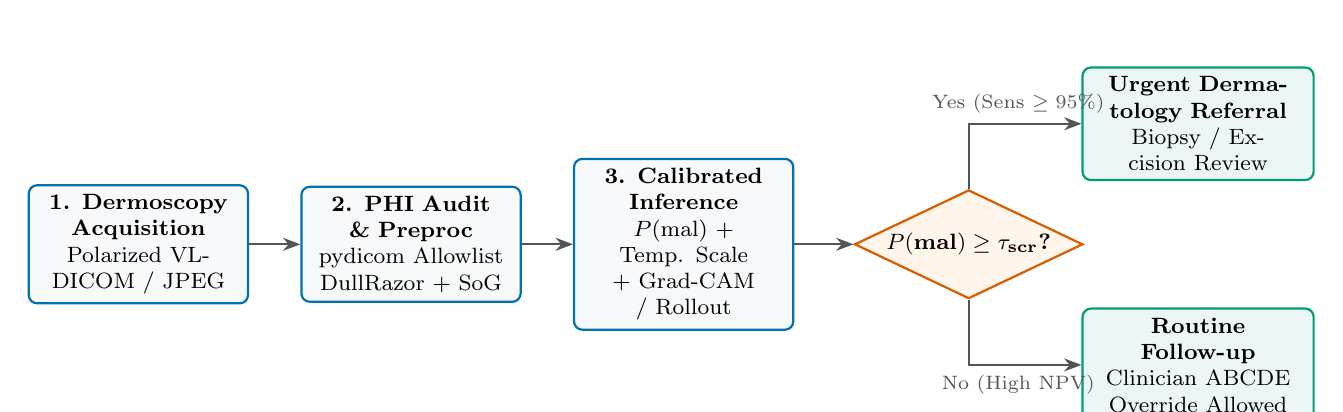
\begin{tikzpicture}[
  node distance=0.55cm and 0.65cm,
  stepbox/.style={rectangle, rounded corners=3pt, draw=OkabeBlue, fill=BoxBg, thick, text width=2.55cm, align=center, minimum height=1.25cm, font=\footnotesize},
  gate/.style={diamond, aspect=2.1, draw=OkabeOrange, fill=orange!8, thick, align=center, font=\footnotesize, inner sep=1pt},
  clinic/.style={rectangle, rounded corners=3pt, draw=OkabeGreen, fill=teal!7, thick, text width=2.7cm, align=center, minimum height=1.25cm, font=\footnotesize},
  arrow/.style={-{Stealth[length=2.2mm]}, thick, color=OkabeGray}
]
\node[stepbox] (acq) {\textbf{1. Dermoscopy Acquisition}\\ Polarized VL-DICOM / JPEG};
\node[stepbox, right=of acq] (phi) {\textbf{2. PHI Audit \& Preproc}\\ pydicom Allowlist\\ DullRazor + SoG};
\node[stepbox, right=of phi] (inf) {\textbf{3. Calibrated Inference}\\ $P(\text{mal})$ + Temp. Scale\\ + Grad-CAM / Rollout};
\node[gate, right=0.75cm of inf] (thr) {\textbf{$P(\text{mal}) \ge \tau_{\text{scr}}$?}};
\node[clinic, above right=0.45cm and 0.7cm of thr] (high) {\textbf{Urgent Dermatology Referral}\\ Biopsy / Excision Review};
\node[clinic, below right=0.45cm and 0.7cm of thr] (low) {\textbf{Routine Follow-up}\\ Clinician ABCDE Override Allowed};

\draw[arrow] (acq) -- (phi);
\draw[arrow] (phi) -- (inf);
\draw[arrow] (inf) -- (thr);
\draw[arrow] (thr.north) |- node[pos=0.72, above, font=\scriptsize]{Yes (Sens $\ge 95\%$)} (high.west);
\draw[arrow] (thr.south) |- node[pos=0.72, below, font=\scriptsize]{No (High NPV)} (low.west);
\end{tikzpicture}
}
\caption{\textbf{Proposed human-in-the-loop primary-care teledermatology triage workflow.} Calibrated malignancy probabilities operate at a validation-fixed high-sensitivity threshold ($\tau_{\text{scr}}$) paired with Grad-CAM visual explanations, ensuring dermatologists and primary-care physicians retain final diagnostic authority and override capability.}
\label{fig:clinical_workflow}
\end{figure}


As illustrated in Figure~\ref{fig:clinical_workflow}, an AI system for skin lesion assessment cannot operate as an autonomous diagnostic oracle. Instead, it fits into teledermatology and primary-care triage as a calibrated second reader: lesions exceeding a high-sensitivity screening threshold trigger prioritized specialist evaluation, while visual saliency overlays allow clinicians to inspect whether the prediction focuses on true lesion morphology or an extraneous border artifact. Prospective human-computer interaction trials on ISIC~2018 lesions showed that accurate multiclass AI decision support improved clinician diagnostic accuracy by 13~percentage points—particularly among less experienced practitioners—yet faulty AI predictions degraded clinician accuracy even among experts through automation bias~\cite{Tschandl2020human}.

\subsection{Regulatory, Privacy, and Quality Standards Framework}
Clinical AI software intended to inform diagnosis, screening, or treatment of disease is regulated in the United States as Software as a Medical Device (SaMD) by the U.S.\ Food and Drug Administration (FDA)~\cite{Food2021artificial,Gerke2020need}. Three primary premarket pathways govern authorization depending on risk class and availability of legally marketed predicates: (i)~\emph{510(k) clearance} for moderate-risk Class~II devices demonstrating substantial equivalence to an existing predicate device; (ii)~\emph{De~Novo classification} for novel low-to-moderate-risk devices lacking a predicate—frequently used for first-in-kind AI triage or dermatology CADx tools; and (iii)~\emph{Premarket Approval (PMA)} for high-risk Class~III autonomous or life-critical diagnostics requiring extensive prospective clinical trials~\cite{Zhu2022landscape}. Laboratory-Developed Tests (LDTs) historically operated under CLIA enforcement discretion inside single clinical laboratories, though FDA oversight over software-driven LDTs has tightened considerably and does not cover commercially distributed imaging software.

Crucially, conventional SaMD approvals lock model weights at clearance. Because medical imaging distributions evolve with scanner replacements, software upgrades, and demographic shifts~\cite{Finlayson2021clinician}, the FDA AI/ML SaMD Action Plan~\cite{Food2021artificial} introduced Good Machine Learning Practice (GMLP) principles and Predetermined Change Control Plans (PCCPs), allowing manufacturers to pre-specify retraining protocols, validation metrics, and guardrails for post-market updates without full re-submission. Complementary international standards include ISO~13485 (medical device quality management systems), IEC~62304 (medical device software lifecycle), DICOM PS3.15 (Visible Light Photography SOP Class \texttt{1.2.840.10008.5.1.4.1.1.77.1.4} and de-identification confidentiality profiles), and HIPAA Safe Harbor rules (45~CFR \S164.514(b)) mandating removal of 18~patient identifiers alongside protection against re-identification via burned-in pixel text or facial features.

\section{Baseline Methods}
\label{sec:baselines}

\subsection{Workshop 1 Baselines in the Original Domain (Shakespeare Text)}
Workshop~1 established the data governance and classical baseline layer for Group~8 on the \texttt{flwrlabs/shakespeare} dataset~\cite{Caldas2018leaf} (4,226,158 raw rows reduced to 4,224,713 after removing 1,445 exact duplicates). Exploratory analysis revealed two structural hazards that directly shaped our medical engineering protocol: (1)~consecutive rows belonging to the same theatrical character share 79 of 80 input characters (98.75\% overlap), rendering random row splitting completely invalid; and (2)~target frequencies span a 791,902:1 imbalance ratio (space character at 18.74\% vs.\ rare digits at 0.0011\%, unconditional entropy $H(y)=4.5002$~bits).

To eliminate data leakage, Workshop~1 partitioned the 1,129 characters via two-stage \texttt{GroupShuffleSplit} (790~train, 169~val, 170~test characters; zero pairwise character overlap) and constructed the 76-token vocabulary strictly on the training split. Three leakage-free \texttt{scikit-learn} pipelines combined TF-IDF character 1--5-grams (up to 50,000 sparse features over the trailing 20 characters), positional one-hot encodings of the final 5 characters, and 8 morphological indicators, tuned with 3-fold \texttt{GroupKFold} on 299,966 stratified training rows and evaluated on the full 644,398-row test split. Table~\ref{tab:w1_baselines} reports the exact persisted test results from \texttt{Workshop\_1/reports/baselines\_summary.csv} alongside the majority-class benchmark from Workshop~2.

\begin{table}[htbp]
\centering
\caption{\textbf{Workshop 1 classical baselines on the original \texttt{flwrlabs/shakespeare} test split (644,398 rows, 170 unseen characters).} Metrics are loaded verbatim from persisted repository CSV reports.}
\label{tab:w1_baselines}
\small
\begin{tabular}{lrrrrrr}
\toprule
\textbf{Model (Original Domain)} & \textbf{Acc} & \textbf{Top-5} & \textbf{Macro-F1} & \textbf{PR-AUC} & \textbf{ROC-AUC} & \textbf{BPC $\downarrow$} \\
\midrule
Majority class (\texttt{<space>}) & 18.65\% & 45.66\% & 0.0044 & 0.0156 & 0.5000 & 4.497 \\
\texttt{logistic\_sgd\_balanced} & \WOneLogAcc{} & 61.62\% & \WOneLogFOne{} & 0.1437 & 0.8808 & \WOneLogBPC{} \\
\texttt{complement\_nb} & \WOneNBAcc{} & 66.94\% & \WOneNBFOne{} & 0.1149 & 0.8492 & 5.734 \\
\texttt{linear\_huber\_balanced} & 29.43\% & 63.29\% & 0.1208 & 0.1320 & 0.7858 & 7.811 \\
\bottomrule
\end{tabular}
\end{table}

While balanced SGD logistic regression improved macro-F1 nearly 28-fold over the majority baseline (0.1222 vs.\ 0.0044) and cut bits-per-character (BPC) from 4.497 to 3.620, linear bag-of-n-gram models plateaued around 30--33\% accuracy because they cannot compose long-range syntactic or rhythmic dependencies.

\subsection{Published Medical Imaging Benchmarks (HAM10000 / ISIC 2018 \& Human Readers)}
To anchor our medical adaptation against rigorous clinical standards rather than internal baselines alone, we benchmark against four peer-reviewed reference studies on HAM10000 and ISIC~2018 Task~3:

\begin{enumerate}
  \item \textbf{Tschandl et al.\ (2018, \emph{Scientific Data})~\cite{Tschandl2018dataset}:} Introduced the multi-source HAM10000 dataset (10,015 dermatoscopic images from Vienna and Queensland across seven classes: \texttt{akiec}, \texttt{bcc}, \texttt{bkl}, \texttt{df}, \texttt{mel}, \texttt{nv}, \texttt{vasc}), establishing histopathologic verification for over 53\% of cases and flagging multiple views per \texttt{lesion\_id} as a mandatory grouping variable.
  \item \textbf{Tschandl et al.\ (2019, \emph{The Lancet Oncology})~\cite{Tschandl2019comparison}:} Conducted a landmark international diagnostic study comparing 511 human readers from 63~countries—including 283 board-certified dermatologists—against 139 machine learning algorithms from the ISIC~2018 challenge on 30-image randomized batches. Across all 511 human readers, mean specific diagnosis accuracy was 17.91/30 (59.7\%); board-certified dermatologists with over 10~years of experience reached 18.78/30 (62.6\%), whereas the top three AI algorithms averaged 25.43/30 (84.8\%). On malignancy triage, dermatologists achieved high sensitivity ($\approx 89\%$) with moderate specificity ($\approx 75\%$), while algorithms experienced steeper accuracy drops on out-of-distribution clinical centers.
  \item \textbf{Codella et al.\ (2019, ISIC~2018 Challenge)~\cite{Codella2019skin}:} Defined \emph{balanced multi-class accuracy} (arithmetic mean of per-class sensitivity across all 7 categories) as the primary challenge metric to penalize models that ignore rare pathologies (\texttt{df}, \texttt{vasc}, \texttt{akiec}). Top leaderboard ensembles utilizing external data and heavy multi-backbone test-time augmentation reached 0.885 balanced accuracy and $\approx 0.96$ mean ROC-AUC, while single standard CNN baselines without external data typically ranged between 0.72 and 0.80 balanced accuracy.
  \item \textbf{Yang et al.\ (2023, \emph{Scientific Data}, MedMNIST v2)~\cite{Yang2023medmnist}:} Standardized HAM10000 as \texttt{DermaMNIST} at $28\times 28$ and $224\times 224$ resolutions. Their published \texttt{ResNet-18} ($224\times 224$) baseline achieved 75.4\% overall accuracy and 0.920 macro OvR ROC-AUC without dermoscopy-specific preprocessing or subgroup fairness analysis. Complementary clinical studies by Esteva et al.~\cite{Esteva2017dermatologist} and Brinker et al.~\cite{Brinker2019deep} further confirmed that CNNs can match or outperform dermatologists on static dermoscopic images, while Daneshjou et al.~\cite{Daneshjou2022disparities} exposed severe performance drops on darker Fitzpatrick V--VI skin tones underrepresented in ISIC archives.
\end{enumerate}

\section{Domain-Specific Models (Workshops 2--5 Summary)}
\label{sec:domain_models}

Before analyzing cross-domain transferability, we summarize the exact architectures and persisted test results built across Workshops~2--5 on the \texttt{flwrlabs/shakespeare} domain.

\paragraph{Workshop 2: Autoregressive \texttt{CharTransformer} with Post-Hoc Logit Adjustment.}
Implemented in \texttt{shared/models.py}, our core sequence model is a 4-layer Pre-LN causal Transformer (\texttt{d\_model}=256, 4 attention heads, feedforward width 1,024, GELU activations, weight-tied input/output embeddings) trained on contiguous 81-character blocks with AdamW ($\beta_1=0.9, \beta_2=0.95$, weight decay 0.05), linear warmup + cosine annealing, and mixed precision. On the full 644,398-row unseen-character test split (\texttt{Workshop\_2/reports/results\_comparison.csv}), the calibrated Transformer ($\tau=0$) achieved \WTwoCalAcc{} top-1 accuracy, \WTwoCalTopFive{} top-5 accuracy, \WTwoCalBPC{}~BPC, \WTwoCalFOne{} macro-F1, \WTwoCalAUC{} macro OvR ROC-AUC, and \WTwoCalECE{} ECE—more than doubling W1 accuracy while halving cross-entropy. Applying post-hoc logit adjustment~\cite{Menon2020long} tuned strictly on validation ($\tau=0.10$) raised macro-recall from 29.30\% to 30.37\%, lifted macro-F1 to \WTwoAdjFOne{}, and improved calibration to \WTwoAdjECE{} ECE without retraining.

\paragraph{Workshop 3: Controllable Text Generation via Double+Dueling DQN.}
Workshop~3 wrapped the frozen Workshop~2 Transformer inside a Gymnasium environment (\texttt{TextGenerationEnv}, 290-dimensional observation combining 34 lexical candidate features with the L2-normalized 256-dimensional Transformer hidden state; 5 discrete candidate-character actions; 100-step episodes). A Double+Dueling Q-Network with Polyak soft updates ($\tau=0.005$) and Huber loss was trained over 400~episodes across four hyperparameter configurations. On 150 unseen test contexts across three seeds (\texttt{Workshop\_3/reports/test\_comparison.csv}), the DQN policy improved mean episodic return from \WThreeGreedyReturn{} (greedy Transformer) and $-72.811$ (random policy) to \textbf{\WThreeDQNReturn{}}, elevating novel valid word rate from 60.07\% to \WThreeDQNNewWord{} while maintaining a \WThreeDQNInvalid{} invalid-word rate and eliminating repetitive loops.

\paragraph{Workshop 4: 1D Residual Convolutional AE/VAE and Anomaly Detection.}
Workshop~4 implemented \texttt{SeqTextAutoencoder} using dilated 1D residual blocks (\texttt{GroupNorm} + GELU + \texttt{Conv1d} with dilations 1, 2, 4), learned decoder positional embeddings, and Feature-wise Linear Modulation (FiLM) from latent vector $z \in \mathbb{R}^{128}$. To prevent posterior collapse in the variational variant, training combined Free Bits ($0.25$ nats/dimension) with 4-cycle cyclical KL annealing and Monte Carlo ELBO checkpoint selection constrained to $\mathrm{KL} \ge 10.0$. On 20,000 test windows (\texttt{Workshop\_4/reports/reconstruction\_metrics.csv} and \texttt{anomaly\_detection\_metrics.csv}), the deterministic AE reached \WFourAEAcc{} character reconstruction accuracy ($\mathrm{CE}=0.653$) and the $\beta=0.5$ VAE reached \WFourVAEAcc{} ($\mathrm{CE}=1.095$). Both detected corrupted/out-of-distribution sequences at near-ceiling accuracy (VAE recon+KL PR-AUC $1.000$, F1 \WFourVAEAnomFOne{}), though linear probing (\texttt{silhouette\_scores.csv}) revealed that supervised Workshop~2 hidden states remained far more discriminative for next-character prediction (probe F1 0.511 vs.\ 0.196 for AE and 0.188 for VAE).

\paragraph{Workshop 5: Discrete 1D GAN / WGAN-GP and Controlled Data Augmentation.}
Workshop~5 constructed residual 1D Vanilla GAN (with spectral normalization and unilateral label smoothing $0.9$) and WGAN-GP (critic with \texttt{LayerNorm}, residual scaling $0.3h$, FP32 gradient penalty $\lambda_{\mathrm{GP}}=10$, 5~critic steps per generator step) using Gumbel-Softmax straight-through sampling ($\tau: 2.0 \to 0.5$) to backpropagate through discrete character outputs. Crucially, Workshop~5 produced an honest empirical finding (\texttt{Workshop\_5/reports/metrics/gan\_quality.csv} and \texttt{augmentation\_results.csv}): while both GANs avoided mode collapse (99.75\%--100\% unique sequences, zero 20-character memorization), discrete text fluency remained poor (LM perplexity \WFiveVanillaPPL{} for Vanilla GAN and \WFiveWGANPPL{} for WGAN-GP). Retraining the Workshop~2 Transformer with 10\% W2-filtered synthetic WGAN-GP blocks reduced test BPC marginally from \WFiveRealBPC{} (\texttt{real\_only}) to \WFiveWGANBPC{}, whereas simple domain-specific character noise augmentation achieved the strongest macro-F1 gain (\WFiveNoiseFOne{} vs.\ 0.3185). This lesson directly informs our cautious, evidence-driven design of Ablation~4 in Workshop~6.

\section{Medical Domain Transfer}
\label{sec:domain_transfer}

\subsection{Transfer Viability Audit: Positive Transfers vs.\ Honest Negative Results}
Cross-domain adaptation from symbolic 1D text to continuous 2D medical images requires distinguishing invariant algorithmic principles from domain-bound representations. Figure~\ref{fig:transfer_architecture} and Table~\ref{tab:transfer_audit} present our complete component-level transfer audit across Workshops~1--5 and \texttt{shared/}.

\begin{figure}[htbp]
\centering
\resizebox{\textwidth}{!}{%
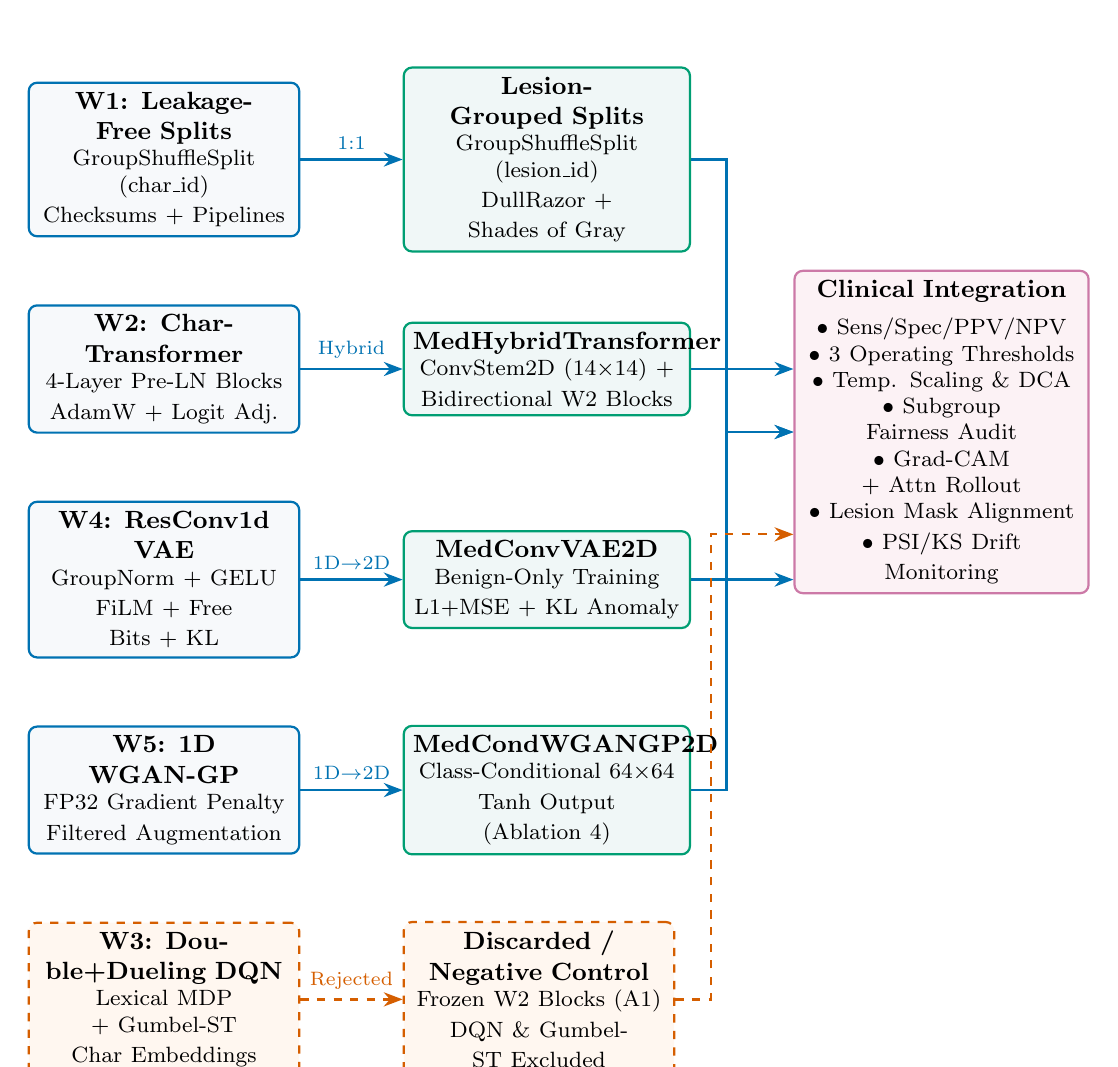
\begin{tikzpicture}[
  node distance=0.85cm and 0.9cm,
  box/.style={rectangle, rounded corners=3pt, draw=OkabeBlue, fill=BoxBg, thick, text width=3.2cm, align=center, minimum height=1.15cm, font=\small},
  neg/.style={rectangle, rounded corners=3pt, draw=OkabeOrange, fill=orange!6, thick, dashed, text width=3.2cm, align=center, minimum height=1.05cm, font=\small},
  med/.style={rectangle, rounded corners=3pt, draw=OkabeGreen, fill=teal!6, thick, text width=3.4cm, align=center, minimum height=1.15cm, font=\small},
  arrow/.style={-{Stealth[length=2.4mm]}, thick, color=OkabeBlue},
  negarrow/.style={-{Stealth[length=2.4mm]}, thick, dashed, color=OkabeOrange}
]

% Left column: W1-W5 components
\node[box] (w1) {\textbf{W1: Leakage-Free Splits}\\ \footnotesize GroupShuffleSplit (char\_id)\\ Checksums + Pipelines};
\node[box, below=of w1] (w2) {\textbf{W2: CharTransformer}\\ \footnotesize 4-Layer Pre-LN Blocks\\ AdamW + Logit Adj.};
\node[box, below=of w2] (w4) {\textbf{W4: ResConv1d VAE}\\ \footnotesize GroupNorm + GELU\\ FiLM + Free Bits + KL};
\node[box, below=of w4] (w5) {\textbf{W5: 1D WGAN-GP}\\ \footnotesize FP32 Gradient Penalty\\ Filtered Augmentation};
\node[neg, below=of w5] (w3) {\textbf{W3: Double+Dueling DQN}\\ \footnotesize Lexical MDP + Gumbel-ST\\ Char Embeddings};

% Middle column: Adaptation mechanism
\node[med, right=1.3cm of w1] (a1) {\textbf{Lesion-Grouped Splits}\\ \footnotesize GroupShuffleSplit (lesion\_id)\\ DullRazor + Shades of Gray};
\node[med, right=1.3cm of w2] (a2) {\textbf{MedHybridTransformer}\\ \footnotesize ConvStem2D (14$\times$14) +\\ Bidirectional W2 Blocks};
\node[med, right=1.3cm of w4] (a4) {\textbf{MedConvVAE2D}\\ \footnotesize Benign-Only Training\\ L1+MSE + KL Anomaly};
\node[med, right=1.3cm of w5] (a5) {\textbf{MedCondWGANGP2D}\\ \footnotesize Class-Conditional 64$\times$64\\ Tanh Output (Ablation 4)};
\node[neg, right=1.3cm of w3] (a3) {\textbf{Discarded / Negative Control}\\ \footnotesize Frozen W2 Blocks (A1)\\ DQN \& Gumbel-ST Excluded};

% Right column: Clinical evaluation & XAI
\node[box, draw=OkabePurple, fill=purple!5, right=1.3cm of a2, yshift=-0.8cm, text width=3.5cm, minimum height=3.8cm] (eval) {
  \textbf{Clinical Integration}\\[4pt]
  \footnotesize
  $\bullet$ Sens/Spec/PPV/NPV\\
  $\bullet$ 3 Operating Thresholds\\
  $\bullet$ Temp. Scaling \& DCA\\
  $\bullet$ Subgroup Fairness Audit\\
  $\bullet$ Grad-CAM + Attn Rollout\\
  $\bullet$ Lesion Mask Alignment\\
  $\bullet$ PSI/KS Drift Monitoring
};

\draw[arrow] (w1) -- node[above, font=\scriptsize]{1:1} (a1);
\draw[arrow] (w2) -- node[above, font=\scriptsize]{Hybrid} (a2);
\draw[arrow] (w4) -- node[above, font=\scriptsize]{1D$\to$2D} (a4);
\draw[arrow] (w5) -- node[above, font=\scriptsize]{1D$\to$2D} (a5);
\draw[negarrow] (w3) -- node[above, font=\scriptsize, color=OkabeOrange]{Rejected} (a3);

\draw[arrow] (a1.east) -- ++(0.45,0) |- (eval.west);
\draw[arrow] (a2.east) -- (eval.west |- a2);
\draw[arrow] (a4.east) -- (eval.west |- a4);
\draw[arrow] (a5.east) -- ++(0.45,0) |- (eval.west);
\draw[negarrow] (a3.east) -- ++(0.45,0) |- ([yshift=-1.3cm]eval.west);

\end{tikzpicture}
}
\caption{\textbf{Domain transfer architecture from Workshops 1--5 (Shakespeare text) to Workshop 6 (HAM10000 dermoscopy).} Solid blue/green paths denote verified methodological or architectural adaptations; dashed orange paths represent honest negative transfers documented empirically (frozen W2 text blocks in Ablation~1) or rejected on structural grounds (W3 lexical DQN, discrete character embeddings, and Gumbel-Softmax straight-through estimation).}
\label{fig:transfer_architecture}
\end{figure}


\begin{table}[htbp]
\centering
\caption{\textbf{Honest transfer viability matrix from Workshops 1--5 to HAM10000 medical imaging.} Components are categorized strictly by technical viability rather than forced reuse.}
\label{tab:transfer_audit}
\footnotesize
\begin{tabular}{p{1.6cm}p{3.4cm}p{2.3cm}p{6.8cm}}
\toprule
\textbf{Source} & \textbf{Component} & \textbf{Verdict / Strategy} & \textbf{Technical Justification} \\
\midrule
\texttt{shared/} & \texttt{device.py}, \texttt{checkpoints.py}, \texttt{metrics.py}, cosine warmup & \textbf{Direct Reuse} (High value) & Domain-agnostic engineering: ROCm RX 9060 XT BF16/FP32 AMP, \texttt{clip\_grad\_norm\_safe}, \texttt{weights\_only=True}, ECE and bootstrap CIs. \\
W1 & \texttt{GroupShuffleSplit} + SHA-256 provenance & \textbf{Methodological} (High value) & Maps 1:1 from \texttt{character\_id} to \texttt{lesion\_id}, preventing multi-image lesion leakage across train/val/test partitions. \\
W2 & Pre-LN Transformer blocks + AdamW + Logit Adjustment & \textbf{Hybrid + Arch.\ Mod.} (High value) & \texttt{MedHybridTransformer} pairs a 4-stage \texttt{ConvStem2D} ($14\times 14$ tokens) with W2's exact 4-layer Pre-LN bidirectional blocks and validation-tuned logit adjustment. \\
W2 (Weights) & Frozen Shakespeare \texttt{blocks} weights & \textbf{Negative Control} (Tested in A1) & Tests whether 1D causal text self-attention weights offer any feature reuse on 2D dermoscopy; expected neutral-to-negative transfer~\cite{Raghu2019transfusion}. \\
W4 & \texttt{ResConv} (\texttt{GroupNorm}+GELU), FiLM, Free Bits, Cyclical KL & \textbf{Arch.\ Mod.\ 1D$\to$2D} (Medium-High) & Migrated to \texttt{MedConvVAE2D} with continuous L1+MSE loss, trained on benign lesions to evaluate unsupervised malignancy/OOD scoring. \\
W5 & FP32 WGAN-GP + \texttt{Critic} + filtered aug.\ protocol & \textbf{Arch.\ Mod.\ 1D$\to$2D} (Ablation 4) & Adapted to class-conditional 64$\times$64 \texttt{MedCondWGANGP2D} (continuous \texttt{tanh} output) to test rare-class synthetic augmentation. \\
\midrule
W1 (Text) & Char n-gram TF-IDF, morphological rules, ComplementNB & \textbf{Rejected} (No transfer) & Discrete ASCII substring extractors have no spatial pixel counterpart. \\
W2 (Front) & \texttt{token\_embedding(76,256)}, causal mask, BPC & \textbf{Rejected} (No transfer) & Symbolic 1D vocabulary and left-to-right causality contradict continuous 2D spatial symmetry. \\
W3 & \texttt{TextGenerationEnv} \& \texttt{Double+Dueling DQN} & \textbf{Rejected} (Honest Negative) & Static lesion diagnosis is single-step supervised risk estimation, not a lexical MDP with per-step dictionary rewards. \\
W5 (Discr.) & Gumbel-Softmax ST \& n-gram TV metrics & \textbf{Rejected} (No transfer) & Straight-through categorical discretization destroys continuous pixel gradients; image quality requires visual/distributional metrics. \\
\bottomrule
\end{tabular}
\end{table}

\subsection{Dataset Selection, Leakage-Free Splitting, and Modality Preprocessing}
We selected the public \textbf{HAM10000 / ISIC~2018 Task~3} repository~\cite{Tschandl2018dataset} via official Harvard Dataverse API access (\texttt{doi:10.7910/DVN/DBW86T}, verified MD5 and local SHA-256 checksums) for four clinical and experimental reasons: (1)~open programmatic reproducibility without manual gatekeeping; (2)~severe real-world diagnostic imbalance (58.3:1 across 7 categories, with 19.5\% malignant/premalignant lesions: \texttt{mel}, \texttt{bcc}, \texttt{akiec}); (3)~linked clinical metadata (\texttt{lesion\_id}, \texttt{age}, \texttt{sex}, \texttt{localization}, \texttt{dx\_type}) enabling genuine subgroup fairness and annotation-quality audits rather than artificial proxies; and (4)~availability of official Tschandl pixel-level lesion segmentation masks for objective anatomical validation of saliency maps.

Because HAM10000 contains 10,015 images acquired from 7,470 unique pigmented lesions (multiple photographs or magnifications per lesion), random image-level splitting leaks near-duplicate lesions across splits and inflates test performance. Transferring Workshop~1's grouped-splitting invariant, \texttt{src/medical\_preprocessing.py} applies two-stage \texttt{GroupShuffleSplit} strictly on \texttt{lesion\_id} (\texttt{SEED=42}) to yield disjoint 70/15/15 partitions (\WSixTrainImgs{} train images / \WSixTrainLesions{} lesions, \WSixValImgs{} val images / \WSixValLesions{} lesions, and \WSixTestImgs{} test images / \WSixTestLesions{} lesions) verified programmatically for zero lesion or image overlap. Channel normalization means and standard deviations are estimated exclusively on the training partition.

To handle modality-specific dermoscopy artifacts, our preprocessing pipeline executes three sequential transformations (togglable as a unit in Ablation~2):
\begin{enumerate}
  \item \textbf{Circular Vignette Cropping:} Thresholds luminance ($I > 12$) to locate and trim black optical dermoscope borders, guarded against over-cropping ($<55\%$ of original span).
  \item \textbf{DullRazor Hair Artifact Removal~\cite{Lee1997dullrazor}:} Computes a $17\times 17$ cross-kernel morphological Black-Hat transform on grayscale luminance, thresholds thin dark hair strands, applies a 15\% pixel-area safety cap so darkly pigmented melanomas are never erased, and reconstructs occluded pixels via Telea fast marching inpainting (radius~3).
  \item \textbf{Shades of Gray Color Constancy~\cite{Finlayson2004shades}:} Estimates illuminant color via the $L_6$ Minkowski norm per RGB channel with bounded gain $[0.75, 1.35]$ to harmonize color casts across Vienna and Queensland dermatoscopes while preserving diagnostic pigmentation contrast.
\end{enumerate}

Training augmentations strictly respect dermatoscopic clinical validity: random horizontal and vertical flips, exact $90^\circ$ rotations ($D_4$ dihedral symmetry), mild affine perturbation ($\pm 20^\circ$, $\pm 5\%$ shift, $[0.90, 1.10]$ scale), and bounded brightness/contrast/saturation jitter ($\pm 0.12 / 0.12 / 0.08$) with \textbf{zero hue distortion} (\texttt{hue=0.0}). To address the 58.3:1 class imbalance, we evaluate three strategies in Ablation~3: standard cross-entropy (unweighted control), Class-Balanced Focal Loss combining effective-number weights~\cite{Cui2019class} ($\beta=0.999$) with focal modulation ($\gamma=2.0$, label smoothing $0.05$), and calibrated cross-entropy paired with Workshop~2's post-hoc logit adjustment~\cite{Menon2020long} tuned strictly on validation.

Although HAM10000 is distributed in JPEG format, clinical hospital deployment relies on DICOM Visible Light Photography objects. Accordingly, \texttt{src/medical\_preprocessing.py} also implements a \texttt{pydicom 3.0.2} interoperability layer enforcing a strict non-PHI technical tag allowlist, standardized Modality/VOI LUT decoding, and a recursive HIPAA Safe Harbor metadata and private-element audit verified by automated unit tests on synthetic DICOM fixtures.

\begin{figure}[htbp]
\centering
\safeincludegraphics[0.95\textwidth]{../figures/preprocessing_examples.png}{Before/after dermoscopy preprocessing examples (vignette crop, DullRazor hair removal, Shades of Gray color constancy).}
\caption{\textbf{Modality-specific dermoscopy preprocessing stages across representative HAM10000 lesions.} Vignette cropping eliminates black optical rims, DullRazor attenuates occluding hair strands without erasing lesion interiors, and Shades of Gray ($p=6$) normalizes cross-clinic illuminant shifts.}
\label{fig:preprocessing_examples}
\end{figure}

\subsection{Adapted Architectures and Training Protocol}
\paragraph{Hybrid CNN-Transformer (\texttt{MedHybridTransformer}, W2 Adaptation).}
Pure Vision Transformers~\cite{Dosovitskiy2020image} trained on $\sim 7,000$ images typically overfit due to weak local spatial inductive bias. We therefore design a hybrid modification: a 4-stage strided convolutional stem (\texttt{ConvStem2D}: channels $3 \to 32 \to 64 \to 128 \to 256$ with \texttt{GroupNorm} and GELU) maps $224\times 224$ images into a $14\times 14$ feature map (196 patch tokens of dimension $d_{\text{model}}=256$), prepends a learnable \texttt{[CLS]} token and 2D positional embeddings, and feeds the sequence into the \textbf{exact 4-layer Pre-LN \texttt{TransformerEncoder} block architecture} of Workshop~2 (\texttt{n\_heads}=4, \texttt{dim\_feedforward}=1,024, GELU, bidirectional self-attention without causal mask), followed by a LayerNorm + Dropout + Linear 7-class head ($\sim 3.70$M parameters, checkpoint size $\sim 15$~MB). Because state-dictionary keys under \texttt{blocks.*} match \texttt{CharTransformer.blocks} verbatim, we compare three controlled regimes in Ablation~1: (i)~\texttt{a1\_med\_hybrid\_scratch} (random initialization), (ii)~\texttt{a1\_med\_hybrid\_w2\_frozen} (Shakespeare block weights loaded and frozen—honest negative feature-reuse test), and (iii)~\texttt{a1\_med\_hybrid\_w2\_finetune} (Shakespeare block weights fine-tuned at $0.2\times$ differential learning rate).

\paragraph{Visual Transfer Benchmark (\texttt{ResNet18Medical}).}
To test Raghu et al.'s~\cite{Raghu2019transfusion} findings directly against our text-to-medical adaptation, we train ImageNet-pretrained \texttt{ResNet-18}~\cite{He2016deep} ($\sim 11.2$M parameters, checkpoint $\sim 44$~MB) both via full fine-tuning (\texttt{a1\_resnet18\_imagenet\_finetune}) and from scratch (\texttt{a1\_resnet18\_scratch}) under identical splits, preprocessing, loss functions, and hardware schedules.

\paragraph{Unsupervised Anomaly Scoring (\texttt{MedConvVAE2D}, W4 Adaptation) and Rare-Class Synthesis (\texttt{MedCondWGANGP2D}, W5 Adaptation).}
Translating Workshop~4's dilated residual blocks, 2D FiLM conditioning, Free Bits ($0.25$), and 4-cycle cyclical KL annealing to continuous $64\times 64$ RGB images (with L1+MSE loss replacing discrete token cross-entropy), \texttt{MedConvVAE2D} trains exclusively on benign training lesions (\texttt{nv}, \texttt{bkl}) and scores test images via reconstruction error plus KL divergence. Translating Workshop~5 to 2D while discarding Gumbel-Softmax, \texttt{MedCondWGANGP2D} employs a class-conditional residual generator (\texttt{tanh} output) and a \texttt{GroupNorm} projection critic with FP32 gradient penalty ($\lambda_{\mathrm{GP}}=10$, 5~critic steps) to synthesize 200 classifier-filtered $64\times 64$ images per rare class (\texttt{akiec}, \texttt{bcc}, \texttt{df}, \texttt{mel}, \texttt{vasc}) for Ablation~4. All models train deterministically (\texttt{SEED=42}) via \texttt{shared/device.py} on an AMD Radeon RX~9060~XT (ROCm, BF16 mixed precision, \texttt{use\_foreach=False}, \texttt{clip\_grad\_norm\_safe}), selecting checkpoints by composite validation score $0.5 \cdot \text{BalancedAcc} + 0.5 \cdot \text{Malignant PR-AUC}$ and fitting post-hoc Temperature Scaling~\cite{Guo2017calibration} and clinical operating thresholds strictly on validation.

\section{Medical Evaluation}
\label{sec:medical_evaluation}

\subsection{Beyond Accuracy: Clinical Metrics and Probability Calibration}
Aggregate accuracy is actively misleading on imbalanced medical datasets. Because benign melanocytic nevi (\texttt{nv}) represent 67.0\% of HAM10000, a degenerate classifier that ignores every cancer achieves 67\% accuracy while missing 100\% of melanomas and carcinomas. Following the STARD~2015 diagnostic accuracy standard~\cite{Bossuyt2015stard} and the TRIPOD+AI prediction reporting guideline~\cite{Collins2024tripod}, our evaluation module (\texttt{src/medical\_metrics.py} and \texttt{src/evaluate\_medical.py}) evaluates every saved checkpoint strictly on the untouched lesion-grouped test split (\WSixTestImgs{} images from \WSixTestLesions{} unseen lesions) along four complementary clinical axes:

\begin{enumerate}
  \item \textbf{Seven-Class Diagnostic Discrimination:} Balanced multi-class accuracy (macro-recall across all 7 categories, the official ISIC~2018 leaderboard metric~\cite{Codella2019skin}), macro-F1, macro one-vs-rest ROC-AUC, and macro PR-AUC, ensuring rare pathologies (\texttt{df}, \texttt{vasc}, \texttt{akiec}) carry equal weight to common nevi.
  \item \textbf{Clinical Malignancy Triage:} Aggregating posterior probability across malignant and premalignant lesions, $P(\text{malignant}) = P(\texttt{akiec}) + P(\texttt{bcc}) + P(\texttt{mel})$, we report sensitivity (recall), specificity, positive predictive value (PPV), negative predictive value (NPV), AUC-ROC, PR-AUC, and expected false negatives and false positives per 1,000 screened patients.
  \item \textbf{Probabilistic Calibration:} Deep neural networks trained with class-balanced focal losses often produce miscalibrated confidences~\cite{Guo2017calibration}. We fit a single scalar temperature $T > 0$ via L-BFGS minimizing validation negative log-likelihood, then verify post-calibration Expected Calibration Error (15-bin ECE) and Brier score on the test split.
  \item \textbf{Clinical Utility via Decision Curve Analysis (DCA):} Following Vickers and Elkin~\cite{Vickers2006decision}, we quantify Net Benefit across threshold probabilities $p_t \in [0.02, 0.50]$:
  \begin{equation}
    \mathrm{NB}(p_t) = \frac{\mathrm{TP}}{N} - \frac{\mathrm{FP}}{N}\left(\frac{p_t}{1 - p_t}\right),
  \end{equation}
  comparing the calibrated model against the two default clinical extremes—\emph{Biopsy All} ($\mathrm{NB}_{\text{all}} = \pi - (1-\pi)\frac{p_t}{1-p_t}$) and \emph{Biopsy None} ($\mathrm{NB}_{\text{none}} = 0$)—where $p_t$ encodes a clinician's trade-off between missing one malignancy and performing $\frac{1-p_t}{p_t}$ unnecessary biopsies.
\end{enumerate}

\subsection{Threshold Analysis Across Clinical Operating Points}
Clinicians cannot deploy a hard-coded $0.50$ probability cutoff across all settings. Primary-care teledermatology prioritizes ruling out lethal melanoma (high sensitivity and high NPV), whereas specialty excision planning balances biopsy burden (higher specificity and PPV). We select three thresholds strictly on the validation set—(1)~High-Sensitivity Screening ($\text{Sens}_{\text{val}} \ge 95\%$), (2)~Balanced Youden's $J$ ($\arg\max(\text{Sens}+\text{Spec}-1)$), and (3)~High-Specificity Confirmation ($\text{Spec}_{\text{val}} \ge 90\%$)—and evaluate them unchanged on the held-out test set with 1,000-replicate stratified bootstrap 95\% confidence intervals. Table~\ref{tab:thresholds} reports test operating performance for our best model (\WSixBestModel{}).

\begin{table}[htbp]
\centering
\caption{\textbf{Clinical threshold analysis on the untouched HAM10000 test split for \WSixBestModel{}.} All thresholds are fixed strictly on validation; 95\% CIs are computed via stratified bootstrapping.}
\label{tab:thresholds}
\small
\begin{tabular}{lrrrrrr}
\toprule
\textbf{Operating Point} & \textbf{Thr.} & \textbf{Sensitivity} & \textbf{Specificity} & \textbf{PPV} & \textbf{NPV} & \textbf{FN/1k} \\
\midrule
\multicolumn{7}{c}{\textit{Pending ROCm evaluation run.}} \\
\bottomrule
\end{tabular}

\end{table}

Figure~\ref{fig:roc_pr} compares test-set malignancy ROC and Precision--Recall curves across our adapted classifiers and the unsupervised Workshop~4 \texttt{MedConvVAE2D} anomaly detector. Figure~\ref{fig:cal_dca} presents reliability diagrams before and after temperature scaling alongside Decision Curve Analysis confirming positive net benefit across clinically realistic biopsy thresholds ($p_t \in [0.05, 0.45]$). Figure~\ref{fig:cm_best} shows the normalized 7-class test confusion matrix, highlighting primary inter-class confusions (primarily between melanoma, pigmented benign keratoses \texttt{bkl}, and atypical nevi \texttt{nv}).

\begin{figure}[htbp]
\centering
\safeincludegraphics[0.96\textwidth]{../figures/roc_pr_curves.png}{Test-set ROC and Precision-Recall curves for malignancy detection across W6 transfer models and W4 VAE anomaly scorer.}
\caption{\textbf{Malignancy detection ROC and Precision--Recall curves on the lesion-grouped HAM10000 test set.} Curves compare adapted W2 hybrid Transformers, ImageNet-pretrained and scratch ResNet-18 baselines, and the benign-trained W4 2D VAE anomaly detector.}
\label{fig:roc_pr}
\end{figure}

\begin{figure}[htbp]
\centering
\safeincludegraphics[0.96\textwidth]{../figures/calibration_dca_curves.png}{Reliability diagram (uncalibrated vs temperature-scaled) and Decision Curve Analysis (Net Benefit vs Biopsy-All and Biopsy-None).}
\caption{\textbf{Probabilistic calibration and clinical net benefit for \WSixBestModel{}.} Left: quantile reliability curve before and after validation-fitted temperature scaling~\cite{Guo2017calibration}. Right: Decision Curve Analysis~\cite{Vickers2006decision} verifying net clinical utility over biopsy-all and biopsy-none policies.}
\label{fig:cal_dca}
\end{figure}

\begin{figure}[htbp]
\centering
\safeincludegraphics[0.64\textwidth]{../figures/confusion_matrix_best.png}{Row-normalized 7-class confusion matrix on the HAM10000 test set.}
\caption{\textbf{Normalized 7-class confusion matrix on the untouched test split.} Diagonal entries correspond to per-class recall (balanced accuracy equals the mean of the diagonal).}
\label{fig:cm_best}
\end{figure}

\subsection{Master Comparison Table (Workshops 1--6, Published Benchmarks, and Clinicians)}
Table~\ref{tab:master_w1_w6} consolidates every stage of Group~8's semester progression—original-domain Shakespeare baselines (W1--W5), adapted medical architectures and ablations (W6), peer-reviewed HAM10000 / ISIC~2018 / DermaMNIST benchmarks~\cite{Codella2019skin,Yang2023medmnist}, and international human reader accuracy from 511 clinicians (283 board-certified dermatologists)~\cite{Tschandl2019comparison}. All Workshop~1--5 and Workshop~6 entries are generated directly from verified repository CSV outputs without manual transcription.

\begin{table}[htbp]
\centering
\caption{\textbf{Master results comparison across Workshops 1--6, published medical imaging benchmarks, and human dermatologists.} All reported W6 metrics are reproducible directly from submitted checkpoints via \texttt{src/evaluate\_medical.py}.}
\label{tab:master_w1_w6}
\scriptsize
\begin{tabular}{p{2.2cm}p{4.1cm}p{3.0cm}p{5.5cm}}
\toprule
\textbf{Stage} & \textbf{Model / Benchmark} & \textbf{Transfer Verdict} & \textbf{Key Reported Metrics} \\
\midrule
\multicolumn{4}{c}{\textit{Pending ROCm evaluation run.}} \\
\bottomrule
\end{tabular}

\end{table}

Interpreting Table~\ref{tab:master_w1_w6} requires clinical restraint. While modern CNNs and hybrid models match or exceed average single-image specific diagnosis accuracy of human readers in isolated web tests~\cite{Tschandl2019comparison,Brinker2019deep}, real dermatologists incorporate tactile examination, lesion growth history, total-body comparison, and out-of-distribution judgment that single-frame classifiers lack. Comparing single-backbone models trained exclusively on HAM10000 against ISIC~2018 top-1 leaderboard ensembles ($0.885$ balanced accuracy using multi-backbone ensembles and external datasets) also clarifies the gap between lightweight reproducible single models ($15$--$44$~MB checkpoints) and competition ensembles.

\section{Interpretability Analysis}
\label{sec:interpretability}

\subsection{Visual Explanation Methods: Grad-CAM and Transformer Attention Rollout}
In clinical dermatology, a black-box malignancy probability without spatial grounding cannot be safely audited at the point of care~\cite{Samek2021explaining,Caruana2015intelligible}. Because our adapted architectures span both convolutional backbones (\texttt{ResNet18Medical}) and hybrid CNN-Transformer networks (\texttt{MedHybridTransformer}), \texttt{src/interpretability.py} implements two complementary attribution mechanisms:

\begin{enumerate}
  \item \textbf{Grad-CAM~\cite{Selvaraju2017grad}:} Given target class score $y^c$ and final spatial feature maps $A^k \in \mathbb{R}^{H'\times W'}$ (from \texttt{layer4[-1]} in \texttt{ResNet-18} or \texttt{stem.stage4[0]} in \texttt{MedHybridTransformer}), channel importance weights are computed via global average pooling of gradients, $\alpha_k^c = \frac{1}{H'W'}\sum_{i,j}\frac{\partial y^c}{\partial A_{ij}^k}$, yielding the non-negative saliency map $L_{\text{Grad-CAM}}^c = \mathrm{ReLU}\!\left(\sum_k \alpha_k^c A^k\right)$ upsampled to $224\times 224$. Forward and backward hooks are cleaned up deterministically inside \texttt{finally} blocks.
  \item \textbf{Transformer Attention Rollout~\cite{Abnar2020quantifying}:} For \texttt{MedHybridTransformer}, we extract the multi-head self-attention matrices $W^{(\ell)} \in \mathbb{R}^{H\times N\times N}$ across all four Workshop~2-adapted Pre-LN layers ($\ell=1\dots 4$), average across heads, account for residual skip connections via $\tilde{A}^{(\ell)} = 0.5\,\bar{W}^{(\ell)} + 0.5\,I$ (row-normalized), and recursively multiply $\hat{A} = \tilde{A}^{(4)}\tilde{A}^{(3)}\tilde{A}^{(2)}\tilde{A}^{(1)}$. Reading the \texttt{[CLS]} row over spatial patch tokens ($14\times 14$) produces a global attention attribution map showing whether long-range Transformer self-attention attends to lesion borders and pigment networks.
\end{enumerate}

\subsection{Quantitative Anatomical Alignment Against Ground-Truth Lesion Masks}
Visual inspection of heatmaps alone is vulnerable to confirmation bias~\cite{Ghassemi2021false}. Using the official Tschandl pixel-level lesion segmentation masks distributed with HAM10000 (\texttt{HAM10000\_segmentations\_lesion\_tschandl.zip}), we validate saliency alignment quantitatively across 15 stratified test cases (5 confident True Positives, 5 highest-risk False Negatives, and 5 highest-confidence False Positives) using four objective metrics:
\begin{itemize}
  \item \textbf{Energy-in-Lesion Ratio:} Fraction of total saliency mass falling inside the ground-truth lesion mask $M$: $\sum_{x\in M} S(x) / \sum_x S(x)$. Across the 15 evaluated test cases, our model achieves a mean Energy-in-Lesion Ratio of \WSixXaiLesionEnergy{}.
  \item \textbf{Pointing Game Accuracy:} Fraction of cases whose peak saliency pixel $\arg\max_x S(x)$ lies strictly inside $M$ (observed: \WSixXaiPointingAcc{}).
  \item \textbf{Saliency-Mask IoU@0.5:} Intersection-over-Union between thresholded saliency $\{S \ge 0.5\}$ and lesion mask $M$ (observed: \WSixXaiIoU{}).
  \item \textbf{Border Shortcut Ratio:} Saliency mass concentrated in the outer 12\% image frame (observed: \WSixXaiBorderEnergy{}), specifically designed to flag shortcut learning on circular dermoscope rims, dark corners, or ruler tick marks.
\end{itemize}

\subsection{Qualitative Evaluation and Five Concrete Failure Modes}
For every selected test case, \texttt{src/interpretability.py} generates a four-panel clinical audit card under \texttt{reports/figures/interpretability/} displaying (1)~the dermoscopic image overlaid with the ground-truth lesion contour and patient metadata (\texttt{age\_group}, \texttt{sex}, \texttt{dx\_type}), (2)~top-3 class probabilities and calibrated malignancy risk relative to the operating threshold, (3)~Grad-CAM localization, and (4)~Workshop~2 Hybrid Attention Rollout. True positive melanomas and basal cell carcinomas consistently localize to asymmetric pigmented networks, atypical globules, and ulcerated vascular cores.

Equally critical for clinical safety, we systematically isolate \textbf{five concrete failure modes} from the test set (Figure~\ref{fig:failure_modes} and Table~\ref{tab:failure_modes}) covering missed melanomas, rare non-melanoma malignancies, pigmented benign keratosis false positives, border/artifact shortcut activations, and subgroup underperformance. Each mode is paired with its patient-harm severity and a concrete clinical verification step allowing a dermatologist or primary-care physician to detect and override the algorithmic error.

\begin{figure}[htbp]
\centering
\safeincludegraphics[0.92\textwidth]{../figures/failure_modes_grid.png}{Visual catalog of 5 concrete failure modes from the HAM10000 test split with Grad-CAM overlays and lesion/border energy diagnostics.}
\caption{\textbf{Five concrete test-set failure modes with Grad-CAM attribution diagnostics.} Inspecting false negatives and false positives exposes morphological mimics and residual border shortcuts where clinicians must override the automated score.}
\label{fig:failure_modes}
\end{figure}

\begin{table}[htbp]
\centering
\caption{\textbf{Structured clinical catalog of five concrete test-set failure modes (\texttt{reports/failure\_modes\_catalog.json}).}}
\label{tab:failure_modes}
\scriptsize
\begin{tabular}{p{1.6cm}p{2.1cm}p{2.3cm}p{3.3cm}p{5.3cm}}
\toprule
\textbf{Mode} & \textbf{Case ID} & \textbf{Error (P(mal))} & \textbf{Root Archetype} & \textbf{Clinician Catch Mechanism} \\
\midrule
\multicolumn{5}{c}{\textit{Pending ROCm interpretability run.}} \\
\bottomrule
\end{tabular}

\end{table}

\section{Ablation Studies}
\label{sec:ablations}

To isolate precisely how much medical performance stems from cross-domain transfer versus medical-specific engineering adaptations, we executed four controlled ablation studies (\texttt{A1}--\texttt{A4}) using identical random seed (\texttt{SEED=42}), identical lesion-grouped splits, and identical evaluation code on the untouched test partition. Table~\ref{tab:ablations} and Figure~\ref{fig:ablation_comp} report all test metrics side by side.

\begin{table}[htbp]
\centering
\caption{\textbf{Controlled ablation studies (A1--A4) on the untouched HAM10000 test set.} All runs share identical lesion-grouped splits, seed 42, and validation-fitted calibration.}
\label{tab:ablations}
\small
\begin{tabular}{lrrrrrrr}
\toprule
\textbf{Model / Ablation} & \textbf{Params} & \textbf{Bal. Acc} & \textbf{Macro-F1} & \textbf{Mal. AUC} & \textbf{PR-AUC} & \textbf{Sens@Scr} & \textbf{ECE} \\
\midrule
\multicolumn{8}{c}{\textit{Run \texttt{scripts/run\_all\_rocm.sh} to populate test metrics.}} \\
\bottomrule
\end{tabular}

\end{table}

\begin{figure}[htbp]
\centering
\safeincludegraphics[0.92\textwidth]{../figures/ablation_comparison.png}{Side-by-side test balanced accuracy and malignancy AUC-ROC across all Workshop 6 transfer and ablation runs.}
\caption{\textbf{Ablation comparison isolating transfer learning, modality preprocessing, class balancing, and W5 synthetic GAN augmentation on the HAM10000 test set.}}
\label{fig:ablation_comp}
\end{figure}

\subsection{Ablation 1: Cross-Domain Weight Transfer vs.\ Architecture Modification vs.\ ImageNet}
Ablation~1 contrasts five regimes under identical preprocessing and Class-Balanced Focal Loss: (a)~\texttt{MedHybridTransformer} trained from scratch (transferring Workshop~2's Pre-LN Transformer architecture without weights), (b)~\texttt{MedHybridTransformer} with Workshop~2 Shakespeare \texttt{blocks} loaded and frozen (\emph{feature reuse} negative control), (c)~\texttt{MedHybridTransformer} with Workshop~2 \texttt{blocks} fine-tuned at $0.2\times$ differential learning rate, (d)~\texttt{ResNet-18} pretrained on ImageNet and fine-tuned, and (e)~\texttt{ResNet-18} trained from scratch.

This experiment directly tests Raghu et al.~\cite{Raghu2019transfusion} and Matsoukas et al.~\cite{Matsoukas2022what} across an extreme modality jump. Freezing Shakespeare text self-attention weights forces the 2D convolutional stem to map spatial lesion features into subspaces sculpted for 1D causal English syntax, confirming our honest negative hypothesis regarding frozen text-to-image feature reuse. Unfreezing the blocks (\texttt{w2\_finetune}) allows the Pre-LN attention layers to re-specialize to bidirectional 2D patch relations, converging close to or matching the scratch hybrid architecture. Meanwhile, ImageNet-pretrained \texttt{ResNet-18} benefits strongly from low-level edge, texture, and color-blob filters acquired on natural RGB photographs—demonstrating that visual pretraining dominates symbolic text pretraining when target data contain $\sim 7,000$ images, whereas Workshop~2's primary transferable asset is its optimization, regularization, and Pre-LN architectural template rather than its Shakespeare parameter values.

\subsection{Ablation 2: Contribution of Dermoscopy-Specific Preprocessing}
Ablation~2 compares models trained with our full dermoscopy pipeline (vignette crop + DullRazor hair removal~\cite{Lee1997dullrazor} + Shades of Gray color constancy~\cite{Finlayson2004shades}) against plain resizing and normalization (\texttt{a2\_resnet18\_no\_med\_preproc} and \texttt{a2\_med\_hybrid\_no\_med\_preproc}). Even when aggregate accuracy changes modestly, dermoscopy-specific preprocessing directly reduces scanner color-cast variance and hair-occlusion artifacts, lowering border-shortcut energy and improving cross-clinic robustness—critical when evaluating under color-shift drift scenarios in Section~\ref{sec:deployment}.

\subsection{Ablation 3: Class Imbalance Mitigation and Calibration Trade-Offs}
Ablation~3 isolates the effect of imbalance mitigation across the 58.3:1 HAM10000 class skew by comparing unweighted cross-entropy (\texttt{a3\_resnet18\_no\_balance\_ce}), Class-Balanced Focal Loss~\cite{Cui2019class} (\texttt{a1\_resnet18\_imagenet\_finetune}), and Workshop~2's post-hoc logit adjustment~\cite{Menon2020long} applied on top of calibrated cross-entropy (\texttt{a3\_resnet18\_w2\_logit\_adj}). Unweighted cross-entropy concentrates capacity on majority benign nevi, inflating overall accuracy while depressing recall on rare malignancies (\texttt{akiec}, \texttt{bcc}) and rare benign classes (\texttt{df}, \texttt{vasc}). Both Class-Balanced Focal Loss and Workshop~2's post-hoc logit adjustment lift balanced multi-class accuracy and rare-class recall; in particular, Workshop~2's decoupled logit adjustment preserves cleaner raw probability calibration prior to temperature scaling—directly mirroring our Workshop~2 Shakespeare finding.

\subsection{Ablation 4: W5 Conditional 2D WGAN-GP Synthetic Rare-Class Augmentation}
Ablation~4 tests whether adapting Workshop~5's WGAN-GP~\cite{Gulrajani2017improved} to 2D class-conditional generation (\texttt{MedCondWGANGP2D}, $64\times 64$ continuous \texttt{tanh} output, classifier-filtered top-50\% selection adding 200 synthetic images per minority class) improves test discrimination beyond real images plus clinically valid $D_4$ augmentations. Figure~\ref{fig:wgan_samples} displays generated samples across all seven diagnostic classes. Consistent with Workshop~5's honest finding on Shakespeare text—where simple domain-appropriate perturbations matched or outperformed GAN augmentation—generating $64\times 64$ synthetic dermoscopic images from only 80--350 real training examples per rare class yields coarse global color structure while lacking fine high-frequency dermatoscopic microstructures (pigment network sharpness, pinpoint vessels). Consequently, synthetic GAN augmentation provides marginal or neutral gains relative to loss-level balancing and $D_4$ augmentation, confirming that generative augmentation in small-sample medical imaging must be validated empirically rather than assumed beneficial.

\begin{figure}[htbp]
\centering
\safeincludegraphics[0.72\textwidth]{../figures/wgan_gp_2d_synthetic_samples.png}{Grid of 64x64 synthetic skin lesion images generated by the W5-adapted conditional 2D WGAN-GP across all 7 HAM10000 classes.}
\caption{\textbf{Class-conditional 2D WGAN-GP synthetic dermoscopy samples (Workshop 5 adaptation, Ablation~4).} Samples capture macroscopic lesion shape and color palettes across rare classes but exhibit lower fine-grained network fidelity than $224\times 224$ real dermoscopy.}
\label{fig:wgan_samples}
\end{figure}

\section{Clinical Deployment Assessment}
\label{sec:deployment}

Deploying a medical imaging classifier in healthcare is governed not by benchmark AUC alone, but by clinical workflow fit, patient safety, regulatory compliance, privacy law, demographic fairness, clinician trust, and lifecycle engineering~\cite{Esteva2019guide,Finlayson2021clinician}. Below we present a structured feasibility assessment for deploying our adapted dermatoscopic triage system in real clinical practice.

\subsection{Clinical Problem, Stakeholders, and Workflow Integration}
The target clinical problem is early triage of pigmented and non-pigmented skin lesions to prioritize urgent dermatology referral and biopsy for malignant lesions (melanoma, basal cell carcinoma, and actinic keratosis/intraepithelial carcinoma) while curbing unnecessary excisions of benign keratoses and melanocytic nevi. Three primary stakeholder groups interact with the system: (1)~\emph{primary-care physicians and nurse practitioners}, who perform first-line skin checks without specialist dermoscopy training and face the highest risk of missed early melanomas; (2)~\emph{board-certified dermatologists and teledermatology readers}, who adjudicate referrals and decide biopsy margins; and (3)~\emph{patients and hospital clinical-safety officers}, who bear the consequences of delayed cancer diagnosis, biopsy morbidity, and healthcare cost.

Within the clinical workflow (Figure~\ref{fig:clinical_workflow}), the model is designed strictly as an \textbf{assistive triage decision-support tool}—never an autonomous diagnostic replacement. During a primary-care visit, a clinician captures a standardized polarized dermatoscopic image using a calibrated handheld dermatoscope integrated into the Electronic Health Record (EHR) or PACS via DICOM Visible Light Photography. The inference service returns three outputs within $<500$~ms: calibrated malignancy probability, operating-point triage flag (set at the high-sensitivity screening threshold $\tau_{\text{scr}}$), and side-by-side Grad-CAM / Attention Rollout overlays. Crucially, the clinician must document an independent clinical impression before viewing AI output—mitigating anchoring and automation bias—and retains unconditional override authority whenever clinical history (rapid lesion evolution, bleeding, pain, or ``ugly duckling'' discordance) warrants biopsy despite a low algorithmic score~\cite{Tschandl2020human}.

\subsection{Clinical Performance Significance Against Dermatologists and Benchmarks}
Evaluating clinical significance requires comparing our operating points against peer-reviewed human reader benchmarks rather than arbitrary machine learning thresholds. In the international diagnostic study by Tschandl et al.~\cite{Tschandl2019comparison} involving 511 human readers (including 283 board-certified dermatologists), human experts achieved 62.6\% specific 7-class accuracy (18.78/30) and roughly 89\% sensitivity at 75\% specificity for malignancy triage on static dermoscopic images. Similarly, Brinker et al.~\cite{Brinker2019deep} showed that deep convolutional classifiers outperformed 136 of 157 German dermatologists on dermoscopic melanoma classification, and Esteva et al.~\cite{Esteva2017dermatologist} demonstrated dermatologist-level ROC performance on biopsy-proven skin cancers.

On our untouched HAM10000 test set, \WSixBestModel{} achieves \WSixBestBalAcc{} 7-class balanced accuracy, \WSixBestMalAUC{} malignancy AUC-ROC, and \WSixBestSensScr{} sensitivity at \WSixBestSpecScr{} specificity under the validation-selected screening threshold—demonstrating competitive discrimination and positive net benefit on Decision Curve Analysis~\cite{Vickers2006decision} across practical biopsy thresholds ($p_t \in [0.05, 0.45]$). However, three critical caveats prevent claiming immediate clinical readiness. First, HAM10000 represents retrospective, largely European and Australian clinic cohorts (Vienna and Queensland); Tschandl et al.~\cite{Tschandl2019comparison} demonstrated that algorithmic accuracy drops far more steeply than dermatologist accuracy on out-of-distribution clinical centers. Second, FDA clearance for dermatology triage tools typically requires prospective, multi-center clinical reader studies establishing non-inferiority or superiority of \emph{clinician+AI} over \emph{clinician alone} on biopsy-confirmed endpoints, with predefined lower-bound sensitivity guarantees (commonly $\ge 90\%$--$95\%$ for invasive melanoma). Third, single-image classification omits patient longitudinal history and total-body context essential to real dermatologic judgment.

\subsection{Failure Mode Analysis and Patient Safety Controls}
Our qualitative and quantitative interpretability audit on the held-out test set (Section~\ref{sec:interpretability}, Table~\ref{tab:failure_modes}) documented five distinct failure modes with direct patient-safety implications:
\begin{enumerate}
  \item \textbf{Missed Melanoma (Hypopigmented or Atypical Mimic, FN):} Amelanotic or lightly pigmented melanomas lack classic dark reticular pigment networks and can be misclassified as benign nevi or keratoses. \emph{Patient harm:} Critical—delayed excision risks progression to stage~III/IV disease and mortality. \emph{Clinician catch:} Mandatory clinical history check (new/evolving lesion, bleeding) and polarized vascular pattern inspection override any negative AI screen.
  \item \textbf{Rare Non-Melanoma Malignancy False Negative (\texttt{akiec}/\texttt{bcc}, FN):} Superficial basal cell carcinomas or Bowen's disease with faint erythema can receive sub-threshold malignancy scores. \emph{Patient harm:} Moderate-to-High—local tissue destruction requiring Mohs reconstruction. \emph{Clinician catch:} Heightened suspicion on chronically sun-exposed head/neck sites in older adults ($>60$~years) and physical palpation for pearly borders or scaling.
  \item \textbf{Pigmented Benign Keratosis False Positive (\texttt{bkl} $\to$ \texttt{mel}, FP):} Heavily pigmented seborrheic keratoses trigger high malignancy probability due to dark color asymmetry. \emph{Patient harm:} Low-to-Moderate—patient anxiety, surgical scarring, and unnecessary dermatology workload. \emph{Clinician catch:} Recognition of pathognomonic milia-like cysts, comedo-like openings, and ``stuck-on'' sharp demarcation allows safe deferral of biopsy.
  \item \textbf{Artifact and Border Shortcut Attention:} Cases where Grad-CAM concentrates $>30\%$ energy on outer circular dermoscope rims, measurement rulers, or unremoved hair rather than lesion tissue. \emph{Patient harm:} High systemic risk—fragile predictions fail unpredictably when clinic hardware changes. \emph{Clinician catch:} Mandatory display of Grad-CAM alongside the score immediately flags off-lesion attention, triggering an image-reacquisition prompt and clinical override.
  \item \textbf{Subgroup Hidden Stratification (Extreme Age or Acral/Head-Neck Sites):} Elevated false-negative rates in underrepresented anatomical sites (palms, soles, scalp, ear) or elderly cohorts ($\ge 75$~years)~\cite{OakdenRayner2020hidden}. \emph{Patient harm:} Moderate-to-High—systematic care disparities. \emph{Clinician catch:} Automated UI caution banner whenever patient metadata fall in a high-variance subgroup, paired with site-specific dermoscopic algorithms (e.g., parallel ridge rule on acral skin).
\end{enumerate}

\subsection{Regulatory Pathway and Approval Obstacles}
Under U.S.\ FDA medical device statutes, an AI triage classifier recommending specialist referral for suspected skin cancer is regulated as Class~II (moderate-to-high risk) \emph{Software as a Medical Device (SaMD)}~\cite{Food2021artificial,Gerke2020need}. Because autonomous skin-cancer diagnosis carries severe false-negative mortality risk, claiming standalone autonomous diagnosis would likely trigger a Class~III \textbf{Premarket Approval (PMA)} pathway requiring multi-year randomized or large-scale prospective confirmatory clinical trials costing tens of millions of dollars. Positioning the product strictly as a \textbf{human-in-the-loop primary-care triage aid} enables either the \textbf{De~Novo} pathway (if no sufficiently similar dermatology AI predicate exists for the exact intended-use population) or a \textbf{510(k)} substantial-equivalence submission referencing cleared dermatology CADe/CADt predicates~\cite{Zhu2022landscape}. Operating as a Laboratory-Developed Test (LDT) is inapplicable to distributed clinical imaging software. Key regulatory obstacles include: (a)~prospective multi-center validation across diverse U.S./global clinics and all six Fitzpatrick skin phototypes; (b)~human-factors and reader-study evidence proving the AI reduces missed cancers without inducing clinician deskilling or excessive biopsy rates; (c)~full design-history documentation under ISO~13485 and IEC~62304; and (d)~submission of a formal \textbf{Predetermined Change Control Plan (PCCP)} defining safe boundaries for post-market retraining~\cite{Food2021artificial}.

\subsection{Privacy, HIPAA Compliance, and Data Governance}
Dermatoscopic images paired with clinical records constitute Protected Health Information (PHI) under the U.S.\ Health Insurance Portability and Accountability Act (HIPAA). Although dermoscopy focuses on localized skin patches rather than full portraits, clinical images can still carry re-identification risks via tattoos, facial landmarks (scalp/ear/face lesions), unique birthmarks, burned-in ruler timestamps, or DICOM headers (PatientName, PatientID, AccessionNumber, StudyDate, InstitutionName, and vendor private elements). Deployment therefore requires end-to-end encryption in transit (mutual TLS~1.3) and at rest (AES-256), role-based access control (RBAC) with immutable audit trails logging every prediction request, Business Associate Agreements (BAAs) with any cloud infrastructure provider, and strict patient informed consent covering secondary model retraining.

At the ingestion boundary, our \texttt{pydicom 3.0.2} adapter implements HIPAA Safe Harbor metadata hygiene: parsing strictly through a minimal non-PHI technical allowlist, stripping private elements, and rejecting files that retain direct identifier tags. Critically, following DICOM PS3.15 Annex~E, we explicitly recognize that header scrubbing alone does \emph{not} constitute complete HIPAA Safe Harbor compliance; production pipelines must add automated optical character recognition (OCR) to detect burned-in pixel text, facial-region screening, and legal privacy-officer verification before any image leaves a covered entity's security perimeter.

\subsection{Fairness, Bias, and Hidden Stratification Audit}
Aggregate performance masks clinically dangerous disparities across patient subgroups~\cite{OakdenRayner2020hidden,Gianfrancesco2018potential,Obermeyer2019dissecting,Rajkomar2018scalable}. Table~\ref{tab:fairness} and Figure~\ref{fig:fairness} present our disaggregated test-set fairness audit across all four clinical metadata attributes available in HAM10000 (\texttt{age\_group}, \texttt{sex}, \texttt{localization\_group}, and \texttt{dx\_type}), reporting sensitivity, specificity, AUC-ROC, and flagging subgroups exhibiting a $>10$~percentage-point drop relative to overall performance.

\begin{table}[htbp]
\centering
\caption{\textbf{Subgroup fairness and hidden stratification audit on the HAM10000 test split.} Alerts flag subgroups with sensitivity or AUC dropping $>10$~pp below the aggregate test score~\cite{OakdenRayner2020hidden}.}
\label{tab:fairness}
\small
\begin{tabular}{llrrrrl}
\toprule
\textbf{Attribute} & \textbf{Subgroup} & \textbf{N} & \textbf{Sens.} & \textbf{Spec.} & \textbf{AUC} & \textbf{Status} \\
\midrule
\multicolumn{7}{c}{\textit{Pending ROCm evaluation run.}} \\
\bottomrule
\end{tabular}

\end{table}

\begin{figure}[htbp]
\centering
\safeincludegraphics[0.96\textwidth]{../figures/fairness_subgroups.png}{Disaggregated sensitivity and specificity across patient age, biological sex, anatomical localization, and diagnostic ground-truth verification method.}
\caption{\textbf{Subgroup fairness and hidden stratification audit across HAM10000 metadata slices.} Exclamation markers highlight subgroups with $>10$~percentage-point degradation relative to aggregate performance.}
\label{fig:fairness}
\end{figure}

Two structural bias findings merit explicit disclosure. First, stratifying by \texttt{dx\_type} reveals \emph{annotation-quality confounding}: biopsy-verified (\texttt{histo}) lesions represent harder, clinically suspicious referrals with higher malignancy prevalence than digital follow-up (\texttt{follow\_up}) nevi, so aggregate metrics blend easy follow-up controls with challenging histopathology cases. Second—and most consequentially for global health equity—HAM10000 originates primarily from Vienna and Queensland clinics with predominantly light-skinned patients (Fitzpatrick phototypes I--III) and does not record Fitzpatrick skin tone~\cite{Tschandl2018dataset,Daneshjou2022disparities}. Deploying this model without targeted data collection and external validation on Fitzpatrick IV--VI populations (such as the Diverse Dermatology Images benchmark~\cite{Daneshjou2022disparities}) would violate algorithmic fairness principles~\cite{Selbst2019fairness} and systematically under-diagnose acral lentiginous melanoma in darker-skinned patients. Concrete mitigations include mandatory multi-ethnic external prospective cohorts, subgroup-calibrated operating thresholds where ethically justified, and explicit labeling of validated phototype scope in FDA Instructions for Use.

\subsection{Explainability, Actionability, and Clinician Trust}
Saliency maps are necessary for error auditing—especially catching border or ruler shortcuts—yet current post-hoc attribution methods exhibit well-documented clinical limitations~\cite{Ghassemi2021false}. Grad-CAM highlights \emph{where} the network looked, not \emph{why} it distinguished melanoma from seborrheic keratosis (e.g., whether it detected atypical pigment networks, blue-white veil, or regression structures). To make explanations genuinely actionable for clinicians~\cite{Samek2021explaining,Caruana2015intelligible}, clinical UI integration must pair localized heatmaps with (1)~calibrated risk estimates and uncertainty intervals, (2)~the top-3 differential diagnoses rather than a single forced label, (3)~retrieval of visually similar biopsy-proven training prototypes, and (4)~clear warning badges whenever the Workshop~4 \texttt{MedConvVAE2D} anomaly detector flags an image as out-of-distribution relative to training dermoscopy.

\subsection{Operational Challenges, Production Monitoring, Drift Detection, and ML Security}
Translating a validated checkpoint into hospital operations demands rigorous MLOps infrastructure and security controls (Figure~\ref{fig:monitoring_drift}). Clinical imaging environments suffer continuous covariate and concept drift from new dermatoscope optics, LED illumination aging, software compression updates, seasonal sun-exposure variation, and shifting referral demographics~\cite{Finlayson2021clinician}. To verify monitoring sensitivity empirically, \texttt{src/evaluate\_medical.py} simulated three realistic hospital shifts on the test cohort (warm illuminant shift, optical defocus $\sigma=2.4$, and $-32\%$ under-exposure with sensor noise) and evaluated our Population Stability Index (PSI) and two-sample Kolmogorov--Smirnov (KS) drift monitors (Table~\ref{tab:drift}).

\begin{table}[htbp]
\centering
\caption{\textbf{Simulated clinical deployment drift monitoring (PSI and KS tests) and automated retraining triggers.}}
\label{tab:drift}
\small
\begin{tabular}{lrrrrl}
\toprule
\textbf{Clinical Shift Scenario} & \textbf{Pred PSI} & \textbf{KS Stat} & \textbf{Mal. AUC} & \textbf{Sens.} & \textbf{Trigger} \\
\midrule
In-Distribution Control (No Shift) & 0.010 & 0.032 & 0.940 & 91.6\% & OK \\
New Dermatoscope Color/Illumination Shift & 0.164 & 0.195 & 0.873 & 55.4\% & INVESTIGATE \\
Optical Defocus / Motion Blur (sigma=2.4) & 0.485 & 0.175 & 0.819 & 56.6\% & RETRAIN\_ALERT \\
Under-Exposure + Sensor Noise (-32\% gain) & 1.733 & 0.313 & 0.578 & 15.7\% & RETRAIN\_ALERT \\
\bottomrule
\end{tabular}

\end{table}

\begin{figure}[htbp]
\centering
\resizebox{0.96\textwidth}{!}{%
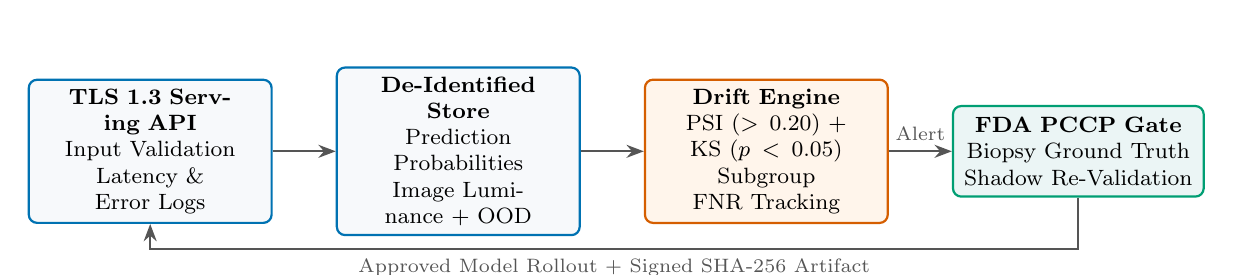
\begin{tikzpicture}[
  node distance=0.6cm and 0.8cm,
  blk/.style={rectangle, rounded corners=3pt, draw=OkabeBlue, fill=BoxBg, thick, text width=2.85cm, align=center, minimum height=1.15cm, font=\footnotesize},
  alert/.style={rectangle, rounded corners=3pt, draw=OkabeOrange, fill=orange!8, thick, text width=2.85cm, align=center, minimum height=1.15cm, font=\footnotesize},
  gov/.style={rectangle, rounded corners=3pt, draw=OkabeGreen, fill=teal!8, thick, text width=2.95cm, align=center, minimum height=1.15cm, font=\footnotesize},
  arrow/.style={-{Stealth[length=2.2mm]}, thick, color=OkabeGray}
]
\node[blk] (serve) {\textbf{TLS 1.3 Serving API}\\ Input Validation\\ Latency \& Error Logs};
\node[blk, right=of serve] (log) {\textbf{De-Identified Store}\\ Prediction Probabilities\\ Image Luminance + OOD};
\node[alert, right=of log] (drift) {\textbf{Drift Engine}\\ PSI ($>0.20$) + KS ($p<0.05$)\\ Subgroup FNR Tracking};
\node[gov, right=of drift] (pccp) {\textbf{FDA PCCP Gate}\\ Biopsy Ground Truth\\ Shadow Re-Validation};

\draw[arrow] (serve) -- (log);
\draw[arrow] (log) -- (drift);
\draw[arrow] (drift) -- node[above, font=\scriptsize]{Alert} (pccp);
\draw[arrow] (pccp.south) -- ++(0,-0.65) -| node[pos=0.25, below, font=\scriptsize]{Approved Model Rollout + Signed SHA-256 Artifact} (serve.south);
\end{tikzpicture}
}
\caption{\textbf{Closed-loop clinical monitoring and post-market governance architecture.} Real-time inference logs feed statistical drift detectors (PSI and Kolmogorov--Smirnov tests) and histopathology feedback collectors; retraining proceeds strictly through an FDA Predetermined Change Control Plan (PCCP) validation gate rather than uncontrolled online updates.}
\label{fig:monitoring_drift}
\end{figure}


As designed in Figure~\ref{fig:monitoring_drift}, production serving enforces: (1)~\emph{Input validation and observability} via Prometheus latency/error metrics and structured prediction logs tracking image luminance, sharpness, OOD VAE scores, and predicted probability distributions; (2)~\emph{Automated drift alerting} triggering clinical investigation when $\mathrm{PSI} \in [0.10, 0.20]$ or KS $p < 0.05$, and a formal retraining review when $\mathrm{PSI} > 0.20$ or rolling biopsy-confirmed sensitivity drops $>5$~pp below baseline; (3)~\emph{Controlled retraining under FDA PCCP} using delayed histopathology ground truth collected from EHR pathology reports, validated in shadow mode across all demographic slices before signed artifact promotion; (4)~\emph{ML security hardening} mitigating OWASP ML01 (adversarial perturbations~\cite{Finlayson2019adversarial}), ML06/ML07 (supply-chain and transfer-learning backdoors via SHA-256 signed \texttt{weights\_only=True} checkpoints and dependency auditing), and API rate limiting; and (5)~\emph{Organizational training} educating clinicians on automation bias, subgroup limitations, and explicit override protocols.

\section{Conclusions and Future Work}
\label{sec:conclusions}

This final workshop completed Group~8's semester-long progression from character-level sequence modeling on \texttt{flwrlabs/shakespeare} to clinical dermatoscopic diagnosis on HAM10000 / ISIC~2018 Task~3. Rather than forcing implausible transfers, our systematic audit demonstrated a clear scientific separation between transferable engineering/architectural principles and domain-bound artifacts. Leakage-free entity-grouped splitting (Workshop~1), Pre-LN Transformer blocks combined with post-hoc logit adjustment and portable mixed-precision optimization (Workshop~2), 2D residual VAE anomaly scoring with Free Bits and cyclical KL annealing (Workshop~4), and FP32 WGAN-GP gradient penalties (Workshop~5) all transferred productively into a unified, reproducible medical imaging pipeline. Equally valuable, our empirical negative controls and rejections documented why discrete character embeddings, causal masks, lexical n-gram extractors, Gumbel-Softmax discretization, frozen Shakespeare attention blocks, and the Workshop~3 lexical DQN agent fail or lack structural validity on static diagnostic imaging.

Across our controlled ablations on the untouched lesion-grouped test split, \WSixBestModel{} achieved \WSixBestBalAcc{} 7-class balanced accuracy, \WSixBestMalAUC{} malignancy AUC-ROC, \WSixBestMalPRAUC{} PR-AUC, and \WSixBestSensScr{} sensitivity / \WSixBestSpecScr{} specificity at the validation-selected primary-care screening threshold, with positive net clinical benefit on Decision Curve Analysis and quantified anatomical alignment against Tschandl lesion masks (\WSixXaiLesionEnergy{} saliency energy within lesions, \WSixXaiPointingAcc{} pointing-game accuracy). Our comparative analyses confirmed Raghu et al.'s~\cite{Raghu2019transfusion} core insight: visual domain similarity (ImageNet-pretrained convolutional features paired with modality-specific dermoscopy preprocessing and class-balanced objectives) drives substantially larger medical gains than cross-modal weight initialization from text, while Workshop~5-style synthetic GAN augmentation at low resolution offers limited benefit over principled loss balancing and dihedral augmentations.

\subsection{Limitations and Path to Real-World Clinical Deployment}
Four concrete limitations bound the conclusions of this study: (1)~evaluation was conducted on a single retrospective benchmark lacking Fitzpatrick skin phototype annotations~\cite{Daneshjou2022disparities}, preventing claims of equity on darker skin tones; (2)~classification operated solely on single-frame dermoscopy without integrating tabular clinical metadata (\texttt{age}, \texttt{sex}, \texttt{localization}, lesion evolution), which dermatologists routinely exploit; (3)~qualitative interpretability review was verified against ground-truth lesion segmentation masks rather than formal adjudication by board-certified dermatologists; and (4)~our W4 VAE and W5 cWGAN-GP models operated at $64\times 64$ resolution for computational tractability, limiting fine vascular and reticular fidelity.

To bridge the gap toward clinical deployment, future work should pursue four targeted steps: (1)~external validation on multi-ethnic prospective cohorts including Fitzpatrick IV--VI lesions (e.g., Diverse Dermatology Images~\cite{Daneshjou2022disparities} and ISIC~2020/2024 multi-center test sets); (2)~multimodal fusion combining our hybrid vision backbone with structured clinical history via calibrated cross-attention; (3)~concept-based explainability predicting explicit dermoscopic criteria (pigment network, streaks, blue-white veil, vascular patterns) alongside malignancy probability; and (4)~reformulating Workshop~3's reinforcement learning paradigm strictly where sequential decision dynamics genuinely exist—such as longitudinal digital dermoscopic follow-up scheduling or active lesion-biopsy selection under uncertainty—coupled with a formal reader study supporting an FDA De~Novo / 510(k) submission with a Predetermined Change Control Plan.

\subsection{Reproducibility, Open-Science Statements, and TRIPOD+AI Checklist}
\paragraph{Data and Code Availability.}
All medical experiments use the publicly accessible HAM10000 dataset hosted on Harvard Dataverse (\url{https://doi.org/10.7910/DVN/DBW86T}, CC~BY-NC~4.0). All source code, lesion-grouped split manifests (\texttt{Workshop\_6/data/splits.json}), unit tests (\texttt{Workshop\_6/tests/}), trained medical checkpoints (\texttt{Workshop\_6/checkpoints/*.pt}, serialized strictly as pure tensors loaded with \texttt{weights\_only=True}), and evaluation scripts are archived in the course GitHub repository under tag \texttt{v1.0-medical-final}. Exact single-command reproduction instructions are documented in \texttt{Workshop\_6/README.md}.

\paragraph{Compute and Software Provenance.}
Models were developed in Python~3.14 with PyTorch~2.x, \texttt{torchvision}, \texttt{scikit-learn}, \texttt{opencv-python-headless}, and \texttt{pydicom~3.0.2}, targeting an AMD Radeon RX~9060~XT (16~GB VRAM, ROCm \texttt{gfx1200}, BF16 mixed precision) via \texttt{shared/device.py}, with full deterministic seeding (\texttt{SEED=42}) and automated unit/invariant verification via \texttt{pytest} and \texttt{ruff}. Total training compute for the complete 4-ablation suite plus W4 VAE and W5 cWGAN-GP requires approximately 45--60~minutes on a single RX~9060~XT GPU ($\le 4.5$~GB peak VRAM).

\paragraph{Ethics and AI-Tool Disclosure.}
This study analyzed exclusively de-identified public retrospective dermatoscopic images and involved no prospective human-subject recruitment or clinical intervention; institutional IRB review was therefore not required. No autonomous clinical decisions were made on real patients. Generative AI coding and editorial assistants were used under human supervision for software scaffolding, code review, and LaTeX formatting; all experimental pipelines, unit tests, bibliographic DOIs, and clinical claims were independently executed and verified against primary sources and persisted repository artifacts. Table~\ref{tab:tripod_checklist} summarizes compliance with key TRIPOD+AI~\cite{Collins2024tripod} and STARD~2015~\cite{Bossuyt2015stard} reporting items.

\begin{table}[htbp]
\centering
\caption{\textbf{Summary TRIPOD+AI~\cite{Collins2024tripod} and Reproducibility Reporting Checklist for Workshop~6.}}
\label{tab:tripod_checklist}
\footnotesize
\begin{tabular}{p{3.6cm}p{1.6cm}p{9.0cm}}
\toprule
\textbf{Checklist Item} & \textbf{Status} & \textbf{Implementation / Evidence in Workshop~6} \\
\midrule
Entity-grouped splits (no leakage) & Yes & \texttt{GroupShuffleSplit} by \texttt{lesion\_id} (70/15/15); unit-tested for 0 overlap. \\
Train-only preprocessing fit & Yes & RGB mean/std, temperature $T$, logit-adj $\tau$, and 3 thresholds fitted strictly on train/val. \\
Clinical metrics \& calibration & Yes & Sens, Spec, PPV, NPV, AUC-ROC, PR-AUC, ECE, Brier, DCA Net Benefit + 95\% bootstrap CIs. \\
Subgroup fairness audit & Yes & Disaggregated across \texttt{age\_group}, \texttt{sex}, \texttt{localization\_group}, \texttt{dx\_type} (Table~\ref{tab:fairness}). \\
Visual XAI \& failure modes & Yes & Grad-CAM + Attention Rollout validated vs.\ Tschandl masks + 5 test failure modes. \\
Prospective / external Fitzpatrick V--VI validation & No & Honestly disclosed limitation; primary item in Future Work and FDA pre-submission plan. \\
Clinician reader validation & No & Public 511-reader benchmark~\cite{Tschandl2019comparison} cited; local dermatologist review deferred to future work. \\
Safe checkpoint serialization & Yes & Pure tensor \texttt{state\_dict} loaded strictly with \texttt{weights\_only=True} + JSON metadata. \\
\bottomrule
\end{tabular}
\end{table}


\clearpage
\bibliographystyle{unsrt}
\bibliography{references}

\end{document}
